\documentclass[12pt,upcase]{mitthesis}
\usepackage{amsmath}
%\newcommand{\angstrom}{\textup{\AA}}
\usepackage{microtype}
\usepackage{graphicx}
\graphicspath{{./images/}}
%\usepackage{multirow}
\usepackage{rotating}
\usepackage{natbib}
\usepackage{url}
\usepackage{booktabs}
\usepackage{makecell}
\usepackage{graphicx, float}            % Graphics/Images.
\usepackage{pgfplots, tikz}             % Drawing/graphing tools.
\usetikzlibrary{
    calc,                   % Calculating right angles and more.
    angles,                 % Drawing angles within triangles.
    arrows.meta,            % Latex and Stealth arrows.
    quotes,                 % Adding labels to angles.
    positioning,            % Relative positioning of nodes.
    decorations.markings,   % Adding arrows in the middle of a line.
    patterns,
    arrows,
    shapes,
    shapes.geometric,
    cd,
    hobby,
    babel
}                                       % Libraries for tikz.
\pgfplotsset{compat=1.9}                % Version of pgfplots.
\usepackage[]{pdfpages}
% for line numbers comment the next two lines before final submission
\usepackage{lineno}
\linenumbers*[1]
% use fancyhdr, to enable page style stuff (below)
\usepackage{fancyhdr}
\setlength{\headheight}{15.2pt}
\renewcommand{\headrulewidth}{0pt}

\pagestyle{plain}
\usepackage{import}                     % Import external files.
\usepackage[subpreambles=false]{standalone}      % Complileable sub files.
\begin{document}
%\include{cover}
%% !TEX root = Thesis.tex
% put this as first line (commented) of every file

\begin{titlepage}
\begin{center}
\vspace*{1cm}

{\Large Title}

\vspace{1.5cm}

BY

\vspace{1.5cm}

SAURAV ARYAL\\
B.S. UNIVERSITY OF WHEREVER (May 2009)\\
M.S. UNIVERSITY OF WHEREVER ELSE (December 2011)

\vfill

SUBMITTED IN PARTIAL FULFILLMENT OF THE REQUIREMENTS\\
FOR THE DEGREE OF DOCTORATE OF PHILOSOPHY\\
DEPARTMENT OF PHYSICS AND APPLIED PHYSICS\\
UNIVERSITY OF MASSACHUSETTS LOWELL

\vfill

\end{center}

\noindent\begin{tabular}{ll}
\makebox[4in]{} & \makebox[1.5in]{}\\
\makebox[4in]{\hrulefill} & \makebox[1.5in]{\hrulefill}\\
Author: Your Name & Date\\[4ex]
\end{tabular}

\noindent\begin{tabular}{l}
\makebox[5.7in]{\hrulefill}\\
Thesis Advisor: Dr. Supriya Chakrabarti \\[4ex]
\makebox[5.7in]{\hrulefill}\\
Committee Member: Dr. Timothy Cook \\[4ex]
\makebox[5.7in]{\hrulefill}\\
Committee Member: Dr. Andryi Danylov
\end{tabular}
\end{titlepage}

%\include{acknowledgements}
\include{contents}
%\include{preface} 	% Preface is not part of the standard. I invented it for myself. Use it if you want by uncommenting.

	% Redefine the "plain" pagestyle to have pagenum in the header, right
	\fancypagestyle{plain}{
		\fancyhf{}
		\fancyhead[R]{\thepage}
	}

	\setcounter{page}{1}
	\pagenumbering{arabic}
	\pagestyle{plain}
	
% \documentclass[crop=false,class=mitthesis,oneside,font=12pt]{standalone}
%----------------------------Preamble-------------------------------%
\usepackage{amsmath}
%\newcommand{\angstrom}{\textup{\AA}}
\usepackage{microtype}
\usepackage{graphicx}
\graphicspath{{./images/}}
%\usepackage{multirow}
\usepackage{rotating}
\usepackage{natbib}
\usepackage{url}
\usepackage{booktabs}
\usepackage{makecell}
\usepackage{graphicx, float}            % Graphics/Images.
\usepackage{pgfplots, tikz}             % Drawing/graphing tools.
\usetikzlibrary{
    calc,                   % Calculating right angles and more.
    angles,                 % Drawing angles within triangles.
    arrows.meta,            % Latex and Stealth arrows.
    quotes,                 % Adding labels to angles.
    positioning,            % Relative positioning of nodes.
    decorations.markings,   % Adding arrows in the middle of a line.
    patterns,
    arrows,
    shapes,
    shapes.geometric,
    cd,
    hobby,
    babel
}                                       % Libraries for tikz.
\pgfplotsset{compat=1.9}                % Version of pgfplots.
\usepackage[]{pdfpages}
% for line numbers comment the next two lines before final submission
\usepackage{lineno}
\linenumbers*[1]
% use fancyhdr, to enable page style stuff (below)
\usepackage{fancyhdr}
\setlength{\headheight}{15.2pt}
\renewcommand{\headrulewidth}{0pt}

\pagestyle{plain}
\usepackage{import}                     % Import external files.
\usepackage[subpreambles=false]{standalone}      % Complileable sub files.
\begin{document}
\chapter{Introduction}
% The upper atmosphere of the earth (90 km+, defined in section \ref{sec:str}) is influenced by forcing from below (the lower atmosphere) as well as forcing from above (the sun). The upper atmosphere is in a weak plasma state due to ionization of chemical species by high energy solar radiation. Understanding the processes in the upper atmosphere thus is important. In this thesis, we study the upper atmosphere during two phenomenon: one involving particle entry and the other involving dynamics generated by thermal changes.
The Ionosphere-Thermosphere (IT) system is the region of the Earth's upper atmosphere which is influenced by energy inputs from the sun and the lower atmosphere. The solar inputs are in the form of high energy Ultra Violet (UV) and X-ray radiation; and, the energetic solar particles that gives rise to observable phenomena such as the aurora. The inputs from the lower atmosphere are in the form of various waves and tides that alter the temperature and the composition of the IT system. The IT region has been studied for decades; however, owing to complex non-linear photochemical, electro-dynamical and collisional interactions involving the Earth's magnetic field, the ionospheric plasma, and the thermospheric neutral constituents, it is not completely understood. Understanding the processes in the IT system is important as many satellites, including the International Space Station (ISS) reside here. The compositional and dynamic changes the IT system introduced by sudden deviation in energy inputs (especially solar inputs) could affect our communication systems and expose astronauts to hazardous radiation environments. In addition, studying the Earth's IT system would also act as a starting point in understanding the upper atmosphere of other planets. In this thesis, study of the IT system's response to two different process is conducted; one involving particle entry and the other involving dynamics generated by thermal changes.

\section{Dissertation Outline}

This thesis is focused on observing the IT system using a ground-based multi-spectral imager known as High Throughput \& Multi Slit Imaging Spectrometer (HiT\&MIS). Based on observations, questions on two different phenomena are studied and answered. The first phenomenon involves estimation of the energetics of solar particle entry during an auroral event by multi-spectral measurements. Specifically, the feasibility of using multi-spectral measurement of auroral brightnesses to simultaneously derive energy and flux of the precipitating auroral electrons is addressed. The second phenomenon involves temperature and composition changes in the polar upper atmosphere due to the effects of total solar eclipse and geomagnetic disturbances that lead to atmospheric waves propagating towards the equator. 

In this first chapter, a simplified theoretical background on a planetary atmosphere, the Earth's upper atmosphere and the IT system is given. Also included is information on how the HiT\&MIS observations are tied to the above mentioned phenomena in the IT system. In chapter 2, details on different instruments that were used for this thesis are provided with emphasis on HiT$\&$MIS. Chapter 3 describes how multi-spectral imaging was used to simultaneously derive the energy and flux during an auroral event. Chapter 4 presents the characterization of Traveling Ionospheric Disturbances (TIDs) generated by Atmospheric Gravity Wave (AGWs) observed using multiple instruments. In Chapter 5, conclusions on the thesis questions mentioned in Section \ref{thesis_q}, based on results obtained in Chapter 3 and 4 are provided.

This dissertation contains modified versions of the publications "Derivation of the energy and flux morphology in an aurora observed at mid‐latitude using multi‐spectral imaging"  by \citet{aryal_energy} (Chapter 3) and "Multi-spectral and multi-instrument observation of TIDs following the Total Solar Eclipse of August 21, 2017" by Aryal et al. (submitted, Chapter 4).

 \section{Theory of the Planetary Atmosphere}
% \begin{figure}[htp]
% 	\centering\includegraphics[width=32pc]{planetary_atmos.png}
% 	\caption{Simplified planetary atmosphere in one dimensional plane-parallel geometry.}
% 	\label{fig:atmos}
% \end{figure}
  \begin{figure}[H]
            \centering
            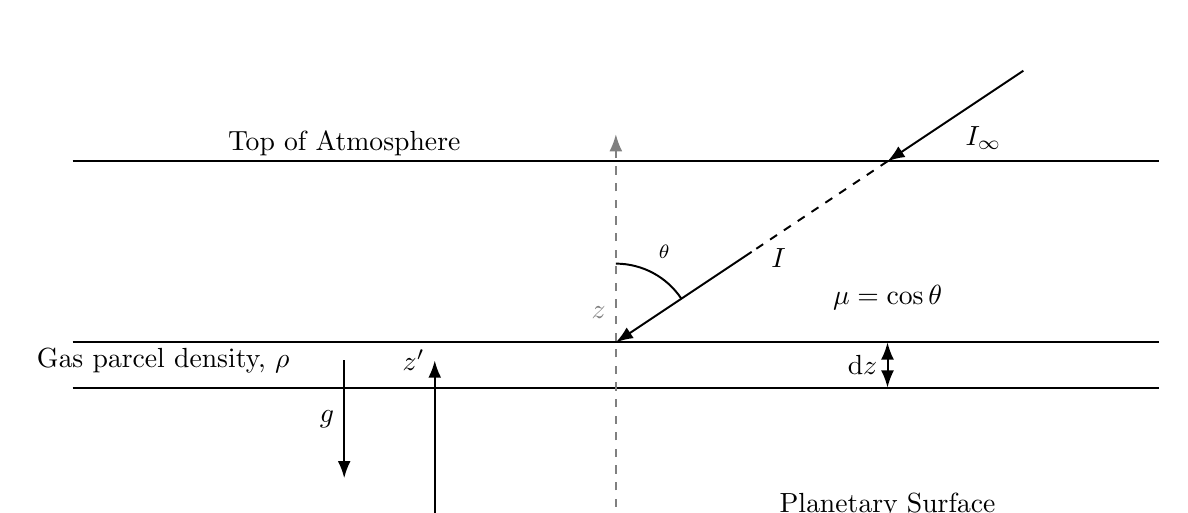
\begin{tikzpicture}[>=Latex, line width=0.25mm,scale=1.15]
                \coordinate (O) at (0,0) {};
                \coordinate (Q) at (0,2) {};
                \coordinate (P) at (3,2) {};
                \draw (-6,-2) to (6,-2);
                \draw (-6,-0.5) to (6,-0.5);
                \draw (-6,0) to (6, 0);
                \draw (-6,2) to (6, 2);
                \draw[dashed] (3,2) to 
                    node [below left=4mm and 3mm] {$I$} (1.5, 1);
                \draw[->] (1.5,1) to (0,0);
                \draw[dashed, ->, gray] (0,-2)
                    to node [above left] {$z$} (0,2.3);
                \draw[->] (4.5,3) to node [below right] {$I_{\infty}$} (3,2);
                \draw[<->] (3,-0.5) to node [left] {$\textrm{d}z$} (3,0);
                \draw[->] (-3, -0.2) to node [left] {$g$} (-3, -1.5);
                \draw[->] (-2, -2) to (-2, -0.2) node [left] {$z'$};
                \node at (-3, 2.2) {Top of Atmosphere};
                \node at (-5, -0.2) {Gas parcel density, {$\rho$}};
                \node at (3, -1.8) {Planetary Surface};
                \node at (3, 0.5) {$\mu= \cos\theta$};
                \pic[%
                    "\scriptsize{$\theta$}",
                    angle eccentricity=1.3,
                    angle radius=1.0cm,
                    -,
                    draw=black
                ]   {angle=P--O--Q};
            \end{tikzpicture}
            \caption{Simplified planetary atmosphere in one dimensional plane-parallel geometry.}
         	\label{fig:atmos}
        \end{figure}
        
This section follows \citet{chamberlain1990theory}, \cite{rees1989physics}, etc. to provide a simplified background on the theory of the planetary atmosphere. Assuming 1D plane-parallel geometry (Figure \ref{fig:atmos}) the pressure (p) gradient on a small parcel of gas with density ($\rho$) contained in small height (dz) of a planet with gravity (g) can be written as:
\begin{equation}
\label{eq:he}
\large
\frac{dp}{dz} = -g(z) \rho.
\end{equation}
This comes from applying Newton's second law to the parcel of gas. Assuming that the gas parcel follows the ideal gas law, the pressure ($p$) can be written as $\rm \frac{\rho}{M} k_B T$, where $k_B$ is the Boltzmann's constant, $T$ is the temperature, and $M$ is the molecular mass of the gas. Replacing the pressure and assuming both the pressure and the temperature to remain constant at all altitude ($z$), equation \ref{eq:he} becomes:
\begin{equation*}
\large
\frac{dp}{dz}= -p \frac{M g}{k_B T} = -\frac{p}{H}  \\
\end{equation*}
\begin{equation*}
\large
\implies \frac{dp}{p}=-\frac{dz}{H}
\end{equation*}
\begin{equation}
\label{eq:p}
\large
\implies p (z)= p(z_{0}) e^{-\frac{z-z_{0}}{H}} \implies n(z)= n(z_{0}) e^{-\frac{z-z_{0}}{H}} ,
\end{equation}
where, H = $\rm \frac{k_B T}{M g}$ is known as the scale height, $z_0$ is the reference altitude and n is the number density. The scale height $H$, is the height at which the pressure (and the number density) drops by $\rm \frac{1}{e}$. For a well-mixed atmosphere, $M$ is the mean molecular weight of all the atmospheric gases. The chemical species diffusively separate for an unmixed atmosphere and each chemical species follow their own scale height $H_j$= $\rm \frac{k_B T}{M_{j} g}$. Here,  $H_j$ and $M_j$ are the scale height and the molecular mass of the j$^{\rm th}$ atmospheric species, respectively.

So far it is assumed that the temperature and the gravity are constant with respect to the atmospheric height. This is an ideal over-simplification as the gravity drops smoothly with height and the temperature changes differently at different layers of the atmosphere (see Section \ref{sec:str}) depending on various inputs into the atmosphere. There are also different chemical and physical processes that transport atmospheric constituents and break hydrostatic equilibrium. Thus, in general, planetary atmospheres are sliced into thin layers where ideal conditions are assumed to hold. 

The column density, N, is defined as the density integrated along a column above a vertical height (z), i.e:
\begin{equation}
\label{eq:N}
\large
N(z) = \int_{z}^{\infty} n(z')~dz'
\end{equation}
Now, using equations \ref{eq:p} and \ref{eq:N}, N becomes:
\begin{equation}
\label{eq:colden}
\large
N(z) =\int_{z}^{\infty} n(z_{0}) e^{-\frac{z'-z_{0}}{H}} dz' \implies N(z) =H n(z),
\end{equation}
which gives an estimation of the scale height in terms of the column density.


\subsection{Radiative Energy Deposition}
\label{sec:edep}
Energy deposition in the atmosphere is mainly governed by two processes involving radiation -- absorption and ionization. The cross-sections of absorption ($\sigma_a$) and ionization ($\sigma$) control where the energy is deposited and are functions of the wavelength of incident radiation. In a plane-parallel atmosphere, for a single chemical species, $j$, with number density $n_j$, that gets illuminated with solar radiation of intensity $I$, the ionization rate $q_j$, is given by the product of the radiation intensity, the ionization cross-section, and the density of the chemical species $j$. In mathematical form, the total ionization rate $q$, is given by:
\begin{equation}
\label{eq:ino}
\large
q(\lambda,~z) = \sum_{j}~I({\lambda},~z)~\sigma_{j}(~\lambda)~n_{j}(z)
\end{equation}
According to Beer's law, the irradiance at height z, considering a single species j, is given by: 
\begin{equation}
\label{eq:beer}
\large
I(\lambda,~z) = I_{\infty}~(\lambda)~e^{-\tau_{j}(\lambda,~z)},
\end{equation}
where I$_\infty$ ($\lambda$) is the irradiance on top of the planetary atmosphere and $\tau_j$ is the optical depth of a single species j. The total optical depth is given by:
\begin{equation}
\label{eq:taua}
\large
\tau(\lambda,~z)~= \sum_{j}~\sigma_{aj}(\lambda)~\int_{z}^{\infty}~n_{j}(z')~dz',
\end{equation}
where $\sigma_{aj}$($\lambda$) is the absorption cross section for the species j. From equations \ref{eq:colden} and \ref{eq:taua}, and considering off-zenith geometry (see Figure \ref{fig:atmos}) with solar zenith angle $\theta$, and defining $\mu$ = cos$~\theta$, the following is obtained: 
\begin{equation}
\label{eq:tau}
\large
\tau(\lambda,~z)~= \sum_{j}\frac{~\sigma_{aj}(\lambda)~N_{j}(z)}{\mu} =~\sum_{j}\frac{~\sigma_{aj}(\lambda)~n_{0j}~H_{j}~e^{-(\frac{z-z_{0}}{H_{j}})}}{\mu}.
\end{equation}
Combining equations \ref{eq:beer} and \ref{eq:tau}, the irradiance at a height z is:
\begin{equation}
\label{eq:irr}
\large
I(\lambda,~z) = I_{\infty}~(\lambda)~ e^{~\sum_{j}\frac{~\sigma_{aj}(\lambda)~n_{0j}~H_{j}~e^{-(\frac{z-z_{0}}{H_{j}})}}{\mu}}.
\end{equation}

\subsection{The Chapman Function}
\begin{figure}[H]
	\centering\includegraphics[width=35pc]{chapman_slm.png}
	\caption{A typical Chapman function in the Earth's atmosphere due to 30 nm solar radiation at various solar zenith angles. Source: \cite{stan_lec1}.}
	\label{fig:chapman}
\end{figure}

Considering only a single atmospheric species j, and radiation incident in the nadir direction ($\theta$ = 0 in Figure \ref{fig:atmos}), using equation \ref{eq:ino} and \ref{eq:irr} the ionization rate is obtained as:
\begin{equation*}
\large
q_{j}(\lambda,~z)=~I_{\infty}~e^{-\tau_{j}~(\lambda,~z)}~\sigma_{j}~n_{0j}~e^{-\frac{z-z_{0}}{H_{j}}}
\end{equation*}
\begin{equation}
\label{eq:chp}
\implies \large
q_{j}(\lambda,~z)=~I_{\infty}~\sigma_{j}~n_{0j}~e^{\big (-\frac{z-z_{0}}{H_{j}}-\tau_{j}~(\lambda,~z) \big )}.
\end{equation}
Equation \ref{eq:chp} is known as the Chapman function for a single species j. Figure \ref{fig:chapman} shows profiles of typical Chapman functions due to 30 nm solar radiation at various solar zenith angles ($\theta$) for a single species. Notice that the ionization peaks around 150 km altitude in this case. Taking derivative of Equation \theequation ~with respect to height and setting it to 0 to optimize, i.e:
\begin{equation*}
\large{
\frac{d q_{j}(\lambda,~z)}{dz}=~ \frac{d[I_{\infty}~\sigma_{ij}~n_{0j}~e^{\big (-\frac{z-z_{0}}{H_{j}}-\tau_{j}~(\lambda,~z) \big )}]}{dz}=~0}
\end{equation*}
\begin{equation*}
\implies \large{
\frac{d q_{j}(\lambda,~z)}{dz}=~ I_{\infty}~\sigma_{ij}~n_{0j}~\Big [\frac{1}{H_{j}} + \frac{\tau_{j}(\lambda,~z)}{H_j}\Big ]~e^{(-\frac{z-z_{0}}{H_{j}}-\tau_{j}~(\lambda,~z))}}{dz}~=0
\end{equation*}
\begin{equation}
\implies \large{
\frac{1}{H_{j}} + \frac{\tau_{j}(\lambda,~z)}{H_j}}~=0 \implies \tau_{j}(\lambda,~z) =1,
\end{equation}
it is found the Chapman function is at $\tau_{j}$($\lambda$, z) =1 for the species j. Thus, the altitude at which $\tau_{j}$($\lambda$, z) =1 is where most of the energy is deposited for a particular species j at a particular wavelength. In an atmosphere with multiple species and the full spectrum of stellar radiation, there can be multiple Chapman peaks, giving rise to Chapman layers.

\section{Earth's Atmosphere}
\subsection{Structure of the Atmosphere}
\label{sec:str}
\begin{figure}[H]
	\centering\includegraphics[width=32pc]{vert_stu.jpg}
	\caption{Vertical structure of the Earth's atmosphere in terms of temperature, density of chemical species and where solar radiation at different wavelengths gets absorbed. Source: \cite{jemrt}.}
	\label{fig:vert_str}
\end{figure}

The Earth's atmosphere is stratified into many different layers (Figure \ref{fig:vert_str}) based on the neutral temperature profile (Figure \ref{TI_temp_var}), how the chemical species mix (Figure \ref{fig:neu_den}) and the differences in dominant physical processes, etc. In terms of the neutral temperature profile, the Earth's atmosphere is divided into the following:
\begin{itemize}
	\item the troposphere (0--15~km in altitude) is where temperature decreases with altitude due to decrease in infrared radiation from the Earth. This is the layer where most of the terrestrial weather occurs. Molecular species (especially N$_2$ and O$_2$) are dominant in the troposphere and all the gases are well-mixed.
	\item The stratosphere (15--50~km) is where there is an increase in temperature when compared to the troposphere as UV radiation gets absorbed by ozone (O$_3$), which is the dominant chemical species. Since the temperature increases with altitude, the stratosphere is thermodynamically stable.
\item  The mesosphere (50--90~km) is where the temperature decreases due to radiative cooling by CO$_2$ and NO. Balloons cannot reach above 40 km because of thinning air and satellites cannot reside here because atmoshpheric drag and gravity are too high compared to the upper atmosphere. Thus, in-situ measurements of the mesosphere is not possible and makes it more difficult to study compared to the other layers.
	\item The thermosphere (90--600~km) is where the temperature increases rapidly due to absorption of high energy solar radiation (UV and X-rays) and lack of cooling mechanism. The number density in the thermosphere is orders of magnitude lower than in the troposphere, and the atomic species start to dominate as molecules are dissociated by solar radiation. High energy solar radiation also ionizes chemical (neutral) species in the thermosphere creating the ionosphere.  Optical emissions (like airglow and aurora) occur in this region of the atmosphere generated by various photochemical and plasma processes.
\item  The exosphere (1000+~km) is marked by extremely low density gas that leak from the Earth's atmosphere. There is no upper boundary of the exosphere as it merges with interplanetary space. The exosphere is sometimes not considered part of the Earth's atmosphere as the conditions are more like space. The lighter gas (mostly hydrogen and helium) in this layer are leaking out into space.
\end{itemize}
\begin{figure}[H]
	\centering\includegraphics[width=35pc]{okl_temp_stru_slr_min_max.png}
	\caption{Temperature structure of the Earth's atmosphere based on MSIS \citep{msie}. Notice sharp rise in temperature in the transition region between the Mesosphere and the Thermosphere after which the temperature plateaus. Source: \cite{stan_lec1} }
	\label{fig:TI_temp_var}
\end{figure}

In terms of mixing, the Earth’s atmosphere is divided into two regions (Figure \ref{fig:neu_den}). 
\begin{itemize}
	\item The heterosphere (up to 100 km) is where all the chemical species are well-mixed due to turbulence. It is dominated by heavier molecules like O$_2$ and N$_2$. 
	\item The homosphere ($>$ 100 km) is where chemical species are not well-mixed due to diffusion and the density structure of each species is determined by mass. That is, the lighter chemical species are found higher in the atmosphere. Thus, the lighter atoms (like O) start being the dominant chemical species. 
\end{itemize}
\begin{figure}[H]
	\centering\includegraphics[width=35pc]{ok_dens_str_neu.png}
	\caption{Neutral density structure of the Earth's atmosphere. In the fully mixed lower atmosphere, the neutral species density have the same scale height, for the unmixed upper atmosphere each species different scale heights and start seperating. Source: \cite{stan_lec1}}
	\label{fig:neu_den}
\end{figure}

In terms of differences in dominant physical processes, the Earth's atmosphere is divided into: 
\begin{itemize}
	\item the lower atmosphere (0-15 km), which is dominated by turbulence and decrease in temperature with increasing heights. 
	\item The middle atmosphere (15-90 km) which is dominated by turbulence and neutral dynamics, but can also effected by very high energy (1 MeV+) solar particles.
	\item The upper atmosphere (90 km and above) which is the focus of this thesis. High energy solar radiation (UV and X-rays) and plasma processes dominate this region. However, it is also influenced by the lower atmospheric tides and waves. 
\end{itemize}
Since the upper atmosphere and specifically the IT system is the focus of this thesis, the rest of the description provided in this chapter is on the upper atmosphere.

%%%%
\subsection{Upper Atmosphere}

The upper atmosphere (90 km+) is the first to receive the direct solar radiative energy input (dominant in mid and low latitudes) as well as the solar charged particle input (dominant in higher latitudes) via the magnetosphere. Most of the high energy solar radiation is deposited in the upper atmosphere as the height where the total optical depth, $\tau$ =1 ($\tau$ as defined in equation \ref{eq:taua}) for these wavelengths lie there (Figure \ref {fig:tau1}).  The high energy solar radiation (X-rays and UV) also ionize the neutral constituents present in the upper atmosphere, creating the ionosphere, the ionized part of the upper atmosphere (Figure \ref{fig:iono_layer}). Thus, the upper atmosphere is a mixture of neutral, ions and electrons whose interactions are then affected by the presence of the Earth’s magnetic field. This thesis is focused on the remote sensing of the one specific part of the upper-atmosphere, i.e., the ionosphere and the thermosphere, sometimes regarded as one system and referred to as the IT system.
\begin{figure}[H]
	\centering\includegraphics[width=32pc]{ionosphere_layers.jpg}
	\caption{Different layers of the ionosphere during the day and during night. Source:  Encyclopedia Britannica, Inc.}
	\label{fig:iono_layer}
\end{figure}

\begin{figure}[H]
	\centering\includegraphics[width=35pc]{tau1.png}
	\caption{Heights where the total optical depth, $\tau$ =1, as a function of wavelength.  $\tau$ =1 is where the the maximum absorption of solar radiation occurs. Also shown are the major chemical responsible for the absorbtion. Source: \cite{thomas2002radiative}. }
	\label{fig:tau1}
\end{figure}

\subsubsection{Thermosphere}
\label{therm}
 Thermosphere is the region in the upper-atmosphere of the Earth's ($\sim$ 90-600 km) where the neutral gas density is orders of magnitude lower compared to the sea level (Figure \ref{fig:neu_den}) and the temperature is high (around 1500 K) due to heating from high energy solar radiation and lack of cooling mechanism. The boundary between the mesosphere and the thermosphere is characterized by rapid increase in temperature with increasing altitude (Figure \ref{fig:TI_temp_var}). The low density environment decreases collisional interaction between the atmospheric constituents, and they start diffusing separately unlike in the lower atmosphere. The lighter atomic constituents (for example Oxygen atom, O), which are almost absent in the lower atmosphere when compared to the molecular (for example, Nitrogen, N$_2$ and Oxygen, O$_2$ molecules), become the dominant chemical species (Figure \ref{fig:neu_den}). The reason behind this is two fold- the molecular diffusion time-scale for heavier molecules (like N$_2$ and O$_2$) is faster than the lighter atoms (like O), and the increase in high energy solar radiation in the thermosphere dissociate molecules into lighter atoms. 

% Thermosphere is also where most of the Low Earth Orbit (LEO) satellites, including the International Space Station (ISS) reside. So, studying the thermosphere (and the embeded ionosphere) also helps in quantifying the effects of upper-atmospheric weather (referred as Space Weather hereafter) on expensive satellites as well as health effects on Astronauts. In addition, radio technologies based on satellites (GPS, satellite internet, etc.) could get disrupted by Space Weather. Like terrestrial weather, the long term goal for Space Weather studies is to predict adverse weather before-hand to limit economic damage caused by such events.
%%%%temperature structure plot

%%%Solar spectrum


%%%%%% Absorbtion of solar radiation
% \begin{figure}[H]
% 	\centering\includegraphics[width=35pc]{slr_rd_abs.png}
% 	\caption{Solar energy deposition in the Earth's atmosphere. Notice that most the highest energy radiation (< 200 nm) are absorbed before thy reach 100 km. Plot courtesy of Dr. Stan Solomon, NCAR }
% 	\label{fig:sl_rad_abs}
% \end{figure}

\begin{figure}[H]
	\centering\includegraphics[width=35pc]{thm_dens.png}
	\caption{Density structure of neutral and ionic species in the Earth's atmosphere based on MSIS and IRI climatological models. Notice lighter atoms and ions are only present above $\rm \sim$ 100 km. Source: \cite{stan_lec2}.}
	\label{fig:TI_dens}
\end{figure}

\subsubsection{Ionosphere}
Ionization due to high energy solar radiation plus collisional ionization by energetic particles of the upper atmospheric neutral constituents creates a weakly ionized region known as the ionosphere (about 60-1000 km). Ionosphere, therefore, is the extension of the thermosphere (and upper mesosphere), i.e, the part of the thermosphere that gets ionized by the solar radiation. During the daytime, when the ionizing source (sun's high energy radiation) is incident on the ionosphere, it gets stratified into different layers and extends into the mesosphere. During the night time, the electrons and ions recombine and the plasma density decreases orders of magnitudes but do not go away completely.

\subsubsection{Ionospheric Layers}
Different part of the high energy solar radiation (daytime) ionize different neutral species which leads to ion density peaking at few specific heights making the ionosphere vertically stratified. As discussed in Section \ref{sec:edep}, peak energy at a particular wavelength and for a species is deposited at the altitude where the optical depth, $\tau$ = 1 (Figure \ref{fig:tau1}). Since the full solar (or stellar spectrum) is incident on all of the chemical elements, the total $\tau$ = 1 altitude for all wavelength peaks at different altitudes causing energies to be deposited at peaks altitudes creating Chapman layers. This stratification ionization peaks giving rise to the ionospheric layers. During the night some of the stratified layers vanish due to recombination and absence of an ionizing source (Figure \ref{fig:iono_layer}). The different layers of the ionosphere are:
\begin{itemize}
\item the D-layer is only present during the daytime and extends from the upper mesosphere to the lower thermosphere (around 60-90 km).
\item The E-layer was the first ionospheric layer discovered, and hence was named the Electric-later (or the E-layer). The other layers above and below the E-layer were named going up or down the alphabet (the D-layer is below the E-layer for example). It ranges from around 90 km to 150 km in altitude.
\item F-layer, is the topmost layer of the ionosphere and splits into two layers, F1 and F2, during the daytime. During the night time, the two layers merge into a single F-layer. The altitude range of the F range is from around 150 km to 1000 km.
\end{itemize}

\section{Magnetosphere} 
\label{magne}
The continuous stream of charged particles from the Sun (solar wind) with its embedded magnetic field, known as the Interplanetary Magnetic Field (IMF), hits the Earth and pushes and distorts the Earth's magnetic field. This creates a long cigar-shaped region where charged particle motion is controlled by Earth's magnetic field region, called the magnetosphere, that is connected to the IMF at its edges (see Figure \ref{fig:magnetosphere}). 
\begin{figure}[htp]
	\centering\includegraphics[width=32pc]{magneto.jpg}
	\caption{Magnetosphere of the Earth and associated current systems. Source: \citet{pollock2003role} }
	\label{fig:magnetosphere}
\end{figure}

To understand the magnetosphere, a brief description of basic plasma physics is required. The Lorentz force ($\bf{F}$) on a collection of charge particles with total charge q, moving at a velocity $\bf{v}$, in a magnetic ($\bf{B}$) and a electric field ($\bf{E}$) is given by:
\begin{equation}
\label{eq:lorentz}
{\bf F}~=~\rm q~({\bf E}+~{\bf v}\times{\bf B})
\implies m~\dot{\bf v}~=~\rm q~({\bf E}+~{\bf v}\times{\bf B}).
\end{equation}
From the equation \theequation, it follows that a single charged particle, in absence of a electric field, will gyrate around and drift along a constant magnetic field line (the guiding center) in a helical trajectory with a frequency of $\omega_{c}$ = $\frac{\rm q B}{m}$ , where m is the mass of the charge particle and B is the magnitude of the magnetic field. While the electrons and ions (positive) gyrate in opposite directions, they both drift along the magnetic field in the same direction (see Figure \ref{fig:drift}), this is what gives rise to the Field Aligned Current (FAC). The gyro-radius can then be expressed as: $r_L$= $\frac{v_\perp}{\omega_c}$=$\frac{m~v_\perp}{\rm q~B}$ ; where $v_\perp$ is the velocity perpendicular to guiding center. In addition to gyration, charged particles in the magnetosphere experiences different drift motions (see Figure \ref{fig:drift}). This is not just due to the geometry of the Earth's magnetosphere, but also due to difference in charge and mobility between electrons (negative charge, lighter) and ions (positive charge, heavier) that set up electric fields and currents in the magnetosphere. Some of these magnetospheric current system (like FAC) flow through the IT system.
\begin{figure}[H]
	\centering\includegraphics[width=25pc]{guiding_cntr_drft.jpg}
	\caption{Examples of drift motions that plasma's can undergo in presence of electric and magnetic fields. }
	\label{fig:drift}
\end{figure}

Gyrating charged particle around a magnetic field line have a magnetic moment, $\mu$ = ${I~A}$ , where, I is the average current due to gyration and A is the current's circular area, and so:
 \begin{equation}
 \mu~=~\frac{m~v^2_{\perp}}{2~B},
 \end{equation}which is a magnetic invariant if the magnetic field is changing slowly with time. In such case, the perpendicular energy of the particle, W$_\perp$ = $\frac{m~v^2_{\perp}}{2}$ is proportional to the magnetic field $\bf{B}$. When the particle moves in the region of stronger magnetic field, $v_\perp$ increases to keep $\mu$ invariant and the drift velocity along the guiding center (magnetic field line) $v_\parallel$, has to decrease due to conservation of energy. By defining, cos$~\alpha$ =$\frac{{\bf v\cdot B}}{v~B}$; where $\alpha$ is known as the pitch angle, the angle between the particle's velocity and the magnetic field.  When the pitch angle reaches 90$^\circ$, the particle gets reflected and this phenomenon is known as magnetic mirroring. Because of the Earth's magnetic field geometry, only particles with mirror points deep into the earth atmosphere can be lost into upper atmosphere, within an area known as the loss cone. These particles that get lost into the Earth's upper atmosphere give rise to auroras. In some region of the magnetosphere magnetic mirroring causes particles to get trapped within regions known as Van-Allen radiation belts. As electrons and protons have different mass (and hence different kinetic energy), there are two Van-Allen belts.
 
Electrical attraction between heavier ions and lighter electrons causes the plasma to re-distributes such that they behave like neutrals by canceling out charges beyond a certain distance. This screen out external electric fields over a characteristic distance known as the Debye length, $\lambda_d$ = $\sqrt{\frac{\epsilon_0~k_{B}~T_{e}}{n~e^2}}$; where $\epsilon_0$ is the electrical permittvity, k$_B$ is the Boltzmann's constant, T$_e$ is the electron temperature n is the electron number density.  In the Earth's ionosphere, the plasma is assumed to be nearly quasi-neutral (equal number of positive and negative charges) and in such case the Debye length is a measure of the distance scale over which positive and negative species act separately.

Plasmas in the Earth's upper atmosphere follow the Maxwell's equation in presence of both magnetic and electric fields:

\begin{equation}
\nabla\cdot \bf{E}~=~\frac{\rho_e}{\epsilon_0}
\end{equation}
\begin{equation}
\nabla \times {\bf E}~= -~\frac{\partial {\bf B}}{\partial t}
\end{equation}

\begin{equation}
\nabla\cdot \bf{B}~=~0
\end{equation}
\begin{equation}
\nabla \times B~=~\mu_{0}{\bf J}+\frac{1}{c^2}\frac{\partial \bf{E}}{\partial t},
\end{equation}
as well as the continuity equation,
\begin{equation}
\label{conti}
\frac{\partial n_{j}}{\partial t}+\nabla\cdot(n_{j}{\bf u}_{j})= P_j-L_j
\end{equation}

and the Ohm's law, ${\bf J}=\sigma {\bf E}$, where $\bf J$ is the current density, $\sigma$ is the conductivity tensor, and $\mu_0$ is the permeability of free space. $P_j$, $L_j$, $n_j$ and ${\bf u}_j$ are the production rate, loss rate, number density and velocity of species j. In the ionosphere, the production and loss rates are also coupled with the neutrals via ionization and recombination, respectively. 
\section{Ionosphere-Thermosphere (IT) system}
The thermosphere together with the charged portion of the upper atmosphere, i.e. the ionosphere, are coupled together via collision and production and loss processes. Thus, this coupled part of the upper atmosphere is known as the Ionosphere-Thermosphere (IT) system. In the lower portions of the IT, the density of the neural species are high enough to get affected by the neutral dynamics (weather) at lower altitudes. Hence, the IT system is influenced by forcing from above (sun) and below (tropospheric weather). Thus making it an ideal laboratory to study the solar-terrestrial interaction.
%\subsection{Why is IT hot ?}%I dont think you need to make a subsection out of it... just another paragraph will probably suffice. Sunip.

As mentioned in Section \ref{therm}, the thermosphere is characterized by rapid increase in temperature at its lower boundary. The ionization processes that create the ionosphere also creates an abundance of free energetic (hot) electron and ions which in-turn heat the neutral species (Figure \ref{fig:therm_heat}) collisionally. Auroral particle precipitation which occur generally in the higher latitudes also have similar heating effect. Such event cause frictional heating known as Joule heating due to enhancement of ionospheric currents.  In addition, various photochemical reaction in the thermosphere contribute in heating the ions and neutrals. Most of the cooling in the atmosphere occurs via radiation, which is dominated by radiation from CO$_2$ and NO. However, in the thermosphere the density of CO$_2$ and NO is orders of magnitude lower compared to the lower atmosphere and so the cooling rate is slow and thus the thermosphere remains hot. 
\begin{figure}[H]
	\centering\includegraphics[width=32pc]{thrm_heat.png}
	\caption{Overview of the thermospheric heating processes. Source: Dr. Stan Solomon, NCAR/UCAR.}
	\label{fig:therm_heat}
\end{figure}


\section{Magnetosphere-IT (MIT) system}
As discussed in Section \ref{magne}, the IT system cannot be de-coupled from the magnetosphere as the the Earth's magnetic field interacts with the ionosphere and vice versa. Their specific interaction is dictated by the geometry of the magnetic field lines at ionospheric heights. Around the magnetic equator, at ionospheric heights, the Earth's magnetic fields are nearly parallel to the surface of the Earth; while near the poles, they are nearly perpendicular. The interaction of plasma with the magnetosphere in conjunction with the co-rotation of the Earth also gives rise to various magnetospheric and ionospheric current system.  In addition, ejection or enhancement of earth-bound solar plasma due to magnetic activities on the sun can also cause changes to the Earth's magnetospheric structure. Furthermore, solar flares, which are sometimes related to plasma ejection events on the sun, can suddenly increase ionization causing perturbations in the magnetic fields at ionospheric heights. Additionally, various magneto-sonic waves, which effect the ionospheric plasma, can also disturb the IT system. In general, these coupling are non-linear in nature and can cause long term (days) Space Weather events that changes the properties of not only the ionosphere but also the thermosphere.

\subsection{MIT coupling}
To study the effect of MIT coupling, two examples are provided below. In the polar region of the Earth, the orientation of the magnetic field lines are almost perpendicular to the Earth's surface and carry the Field Aligned Currents (FACs) with them into and out of the ionosphere (Figure \ref{fig:mit_cpl_p}). The FACs are the manifestation of plasma gyration and magnetic mirroring drift as discussed in Section \ref{magne}. The FACs can also be enhanced by energetic plasma particles that get accelerated into the upper atmosphere via the magnetic field lines during magnetic re-connection events. The plasma carried by the FAC that are in the loss cone get lost into the ionosphere give rise to auroras and deposit energy. For the current system to close, the currents brought by the FACs diverge as they flow through the ionosphere and give rise to the Pedersen and Hall currents (Figure \ref{fig:mit_cpl_p}). Each of the associated currents have their characteristic conductivities ($\sigma_P$, Pedersen and $\sigma_H$, Hall conductivity). In the ionosphere these conductivities determine the exact interaction between the Pedersen and Hall currents. Figure \ref{fig:ped_hall} shows different physical regime encountered by FAC at different ionospheric layers. Any perturbation to the magnetic field disturbs these currents and ultimately the IT system, but the exact change depends on the nature of the magnetic disturbance.

\begin{figure}[H]
	\centering\includegraphics[width=35pc]{mit_cpl_i.png}
	\caption{Summary of how the Magnetosphere is coupled to the IT system at higher latitudes. Plasma flows (Field Aligned Current) via the magnetec field into and out of the ionosphere (Pedersen Currents) produces hall currents. Source: \cite{lotko} }
	\label{fig:mit_cpl_p}
\end{figure}
\begin{figure}[H]
	\centering\includegraphics[width=35pc]{ion_hall_ped.png}
	\caption{Summary of how the the electron and ions flowing into the ionosphere (Field Aligned Current) via the magnetec fields interact with the different layers of the ionosphere. This leads to velocity diversion giving rise to the Pedersen and Hall currents in the ionosphere. Source: {lotko} }
	\label{fig:ped_hall}
\end{figure}

In the equatorial region, the interaction between the neutral wind and the ionospheric plasma (changes in conductivity with height) creates the Equatorial Electro Jet (EEJ). The EEJ creates a east-west electric field which interacts with the magnetic field geometry. The magnetic field lines are almost parallel to the Earth's surface in this region (Figure \ref{fig:eia}). By applying $\bf B$ $\times$ equation \ref{eq:lorentz}, it is found that the velocity of plasma is $\frac{{\bf E}\times {\bf B}}{B^2}$, for both electron and ions, this is known as the  ${\bf E}\times {\bf B}$ drift.  Thus, the magnetic-field geometry (parallel to the Earths surface and perpendicular to the EEJ electric field) at the equator lifts the plasma up via  ${\bf E}\times {\bf B}$ drift. These plasma then diffuse down on either side of the equator due to pressure gradient and gravity creating an enhanced dense plasma region on either side of the magnetic equator known as the Equatorial Ionization Anomaly (EIA, Figure \ref{fig:eia}, \cite{immel2006control} ). This processes also creates various plasma instability leading to different ionospheric scintillations. 

These two examples of MIT coupling show how the magnetosphere interacts with the ionosphere and its dependence on the magnetic field geometry. In this thesis, the MIT coupling at the polar region is of particular interest because there was a minor geomagnetic disturbance during HiT\&MIS's observation of airglow brightness perturbations hours after the eclipse. This will be discussed further in Chapter 3. 
\begin{figure}[H]
	\centering\includegraphics[width=35pc]{eia.jpg}
	\caption{The geometry of MIT coupling in the equatorial region that leads to EEJ and EIA. Source: \citet{immel2006control}. }
	\label{fig:eia}
\end{figure}
\subsection{Dynamics and chemistry in the IT system}
\label{dyn_cm}
Neutral gasses are governed by momentum equation defined in Figure \ref{fig:n_mom}, which shows all the terms effecting the neutral wind velocity ${\bf U}$. Most changes in the neutral winds are produced by forcing from below in events such as uplifting of the atmosphere during tsunamis and earthquakes, etc. In general, the neutral wind is altered very little by the plasma (specifically the ions as they are much heavier than electrons), since the plasma densities are orders of magnitude lower than neutral densities at IT heights, and assumed as such. However, neutral winds can get be altered indirectly due to plasma processes. For example, during geomagnetic storms, enhancement in ionospheric currents leads to collisional heating of the neutral atmosphere. Neutral winds (especially vertical winds) cause re-distribution of chemical species leading to alters the photochemistry in the IT system.
\begin{figure}[H]
	\centering\includegraphics[width=35pc]{momentum.png}
	\caption{The neutral momentum equation with physical description of each terms. Source \cite{ingo} }
	\label{fig:n_mom}
\end{figure}

Just like plasmas in equation \ref{conti}, neutral gases also follow the continuity relation (see Figure \ref{fig:n_cont}), which is coupled to the momentum equation via the neutral wind. The neutral continuity equation is also coupled to plasma continuity equation by plasma-neutral collision and via production (ionization) of plasma that leads to loss of neutrals and loss of plasma (recombination) that leads to the production of neutral gases. 
\begin{figure}[H]
	\centering\includegraphics[width=35pc]{neu_cont.png}
	\caption{The neutral continuity equation with physical description of each terms. Source: \cite{ingo} }
	\label{fig:n_cont}
\end{figure}

In addition to the dynamics, changes to IT system is also caused by various photochemical reactions involving both plasma and neutrals. The major types of photochemical reactions taking place in the IT system are:
\begin{itemize}
\item \textbf{Radiative recombination}: X$^+$ + e$^-$ $\rightarrow$ X + photon; the reaction rate is in order of 10$^{-12}$ cm$^3$ s$^{-1}$ .
\item \textbf{Dissociative recombination}: XY$^+$ + e$^-$ $\rightarrow$ X + Y; the reaction rate is in the order of 10$^{-7}$ cm$^3$ s$^{-1}$
\item \textbf{Charge Exchange}: WX$^+$ + YZ $\rightarrow$ WX + YZ$^+$ ; reaction rate depends of the strength of the molecular bond YZ
\end{itemize}

Plasma dynamics is governed by Electro-magnetic forces as defined in Section \ref{magne}, ambipolar diffusion and interaction with neutrals (chemical and collisional) and these interactions are non-linear. The neutral dynamics at IT heights is governed by chemistry and molecular diffusion. Time scales determines which process dominates at different region in absence of external forcings. The time scales of the different process depends on the density structure (and hence the altitude) of the plasma and neutrals. For example, at lower altitudes the heavier molecular ions and neutrals are more abundant, thus during quiet times it is the photochemistry that dominates. However, in the topside of the ionosphere because of lower molecular diffusion time and higher density of O$^+$ compared to other ions and neutrals, its dynamics dominates as electrons also follow O$^+$ velocity via ambipolar diffusion. In the F region of the ionosphere, the time scales of diffusion and chemistry are similar and both processes are important.  These differences in dominant processes in conjunction with difference in solar heating give rise to the "climate" in the IT system.

\begin{figure}[H]
	\centering\includegraphics[width=35pc]{diff_tscale.png}
	\caption{Time scales of various process in the IT system.Source: \cite{ingo}}
	\label{fig:diff}
\end{figure}

\section{IT Climatology}
In general the climatologal variability in the IT system can be divided into predictable direct forcing from the sun that generally effect the ionosphere due to MIT coupling, and predictable forcing due to atmospheric waves and tides that effect the neutral composition and the temperature structure of the thermosphere. It is to be noted that some of the atmospheric tides (e.g., thermal tides) are also driven by the sun. These variabilities lead to compositional and/or thermal changes in the IT system that are predictable and can be thought of as the climate of the IT system. 

\subsection{Solar Forcing}
\begin{figure}[H]
	\centering\includegraphics[width=35pc]{solar_spectrum.png}
	\caption{Typical example of solar spectral irridance incident on top of the Earth's atmosphere (blue). Ratios of variability in irridance between solar max and minimum periods are shown in green. Notice that the high energy radiation ($<$ 100 nm, in UV and EUV) vary orders of magnitude more than the visible and infrared spectrum. Source: \cite{juzeniene2011solar}. }
	\label{fig:solar_spec}
\end{figure}

The blackbody radiation is a radiation pattern emitted by a theoretical black body (Figure \ref{fig:solar_spec}). Black bodies are defined as perfect absorbers of radiation that are in thermal equilibrium with the surrounding. A lot of stars, including our sun, behave similar to a black-body at visible and infrared wavelengths and have a similar emission profile. However, in radio, far and extreme UV (FUV and EUV) and X-rays the emissions from the sun do not follow the black-body spectrum and are far more variable, driven by various processes in the Sun (Figure \ref{fig:solar_spec}). In the IT system, it is the solar X-ray, EUV and FUV that are responsible for ionization and the heating. So, the climatological variability of the IT system is dominated by the variability of high energy solar radiation, which is characterized by the solar cycle. The solar cycle is the periodic variation in the high energy radiation from the sun that is correlated with the number of sunspots and the radiation in the radio waves (Figure \ref{fig:slrcyc}). The F10.7 cm (flux at 10.7 cm radiation) measurement therefore is a proxy to variability of high-energy solar radiation. These variability change the density of neutrals, due to heating or cooling, and plasma due to increase or decrease in ionization. Figure \ref{fig:it_minmax}, shows typical variability in ion and neutral densities at solar minimum and maximum.
\begin{figure}[H]
	\centering\includegraphics[width=35pc]{solar_cycle.eps}
	\caption{The Solar Cycle as characterized by Sun Spot Numbers (SSN). Higher frequency of sunspot represents active solar times. Also shown in blue, starting from 1960s is the solar flux at 10.7 cm (F 10.7). Notice clear coincidence between SSN and solar flux. }
	\label{fig:slrcyc}
\end{figure}
\begin{figure}[H]
	\centering\includegraphics[width=35pc]{slr_minmax_slm.png}
	\caption{Density structure in the IT. Both ion and neutral density increase during the solar max period. Plot courtesy of Dr. Stan Solomon, NCAR }
	\label{fig:it_minmax}
\end{figure}


\subsection{Tidal/ Wave forcing}
The climatological forcings can also be caused by various tides and planetary waves. The rotation of the earth creates a planetary waves, also known as Rossby waves, due to Coriolis force, pressure gradient and conversation of momentum (Figure \ref{fig:n_mom}). Similarly, thermal tides driven due to absorption of solar radiation by O$_2$ in the thermosphere, O$_3$ in the lower mesosphere/ upper stratosphere and water in the troposphere also cause temperature changes. In addition, moon's gravitational pull also cause lunar tides in the atmosphere like the lunar ocean tides, that alter the IT composition and temperature as dictated by the moon's cycle. 

\section{IT variability}
Abrupt change in the forcings into IT system lead to rapid change in the density structure and temperatures of both plasma and neutral species. Like the climatological variations, these can also be divided into the effect of sudden changes to solar and wave forcings. While the climatological effect of the solar cycle is predictable, solar max is characterized by events such as solar flare and Coronal Mass Ejection (CME), and changes in solar wind conditions, etc. These changes in solar wind conditions and the Earth bound CMEs, directly linked to the solar weather, can abruptly change magnetospheric structure, plasma density, etc. In addition, solar flares increase the high energy radiation environment incident on earth, causing increase in ionization on the dayside. While the changes in solar forcings only effect the magnetosphere and ionosphere directly, these can indirectly heat/cool the thermosphere disturbing global circulation patterns and hence thermospheric composition. There are also situations when changes in solar forcing can lead to change in both ionosphere and thermosphere simultaneously and vice versa. For example, during a total solar eclipse, lack of high energy radiation around totality not only decreases photo-ionization but also cools the thermosphere leading to pressure changes and wind blowing into the region of totality. In this thesis, two phenomenon brought about due to solar forcing are studied, one due to a geomagnetic storm and the second due to a total solar eclipse. Both of these events change the photochemistry and collisional interaction between in the IT system modulating the brightness morphologies of the upper atmospheric emissions.

% Figure \ref{fig:a_ther_dyn} shows how changes in geomagnetic condition changes the IT system during solstice. Figure \ref{fig:a_ther_dyn} (top) shows the normal thermospheric circulation, when solar heating in the summer hemisphere heats and expands the thermosphere making the upper atmosphere molecule rich (N$_2$ used as proxy). At higher altitude molecular diffusion dominates, thus, the molecules diffusively seperate and blown by winds into the winter hemisphere. In the winter hemisphere where it is cooler the thermosphere shrink and so do the molecules that then flow into the lower part of the equatorial and summer hemisphere creating a one cell convection pattern. 

% Figure \ref{fig:a_ther_dyn} (bottom) shows the circulation pattern during the same time of the year (solstice) but at geomagnetically active condition. During geomagnetic events, the FACs are also enhanced along with associated Pedersen and Hall currents. In such case, the auroral heating in the winter hemisphere increases the molecular density near the poles too. This causes a two cell circulation pattern as only the mid latitudes are cooler. 

% \begin{figure}[H]
% \centering\includegraphics[width=35pc]{therm_quiet_dyn.png}
% 	\centering\includegraphics[width=35pc]{therm_act_dyn.png}
% 	\caption{Top: Global circulation pattern in the IT system at solstice during geomagnetically quiet time. Bottom: Same as the top but during geomagnetically active times.} }
% 	\label{fig:a_ther_dyn}
% \end{figure}

\section{Emissions in IT system: Airglow and Aurora}


The interaction the ionospheric electrons, called the photo-electrons (produced by photo-ionization)  or secondary electrons (produced my charges particle precipitation), with the neutral and ionized chemical species via collision and/or photo-chemical reactions discussed in Section \ref{dyn_cm}, gives rise to optical emission at different spectral regions in the IT system. 

As mentioned in Section \ref{magne}, most of the energetic particles carried by the solar wind flow around the Earth's magnetic field that is distorted by the IMF, except around the magnetic poles. Around the magnetic poles, the more perpendicular orientation of the Earth’s magnetic field allows solar particles to enter the upper atmosphere of the Earth, either directly through the magnetic cusp (Figure \ref{fig:magnetosphere}) or via MIT coupling. Furthermore, radiation-belt particles can diffuse or get accelerated into the upper atmosphere and enter the IT system, especially during geomagnetic disturbances. Most of these entry of the energetic particles occurs at high latitudes through the loss cone; however, during solar storms (characterized by a sudden increase in speed and density of solar wind particles) particle precipitation can occur even at low and middle latitudes depending on the strength of the storm and the orientation of IMF. These electrons precipitating at high energy collisionally ionize and create secondary electrons. These secondary electrons then produce emissions by collisional excitation and enhancement of photochemical reactions. Similarly, photo-electron produced by solar radiation also lead to emissions in IT system by same collisional and photochemical processes. However, these have different morphology to emissions produced by due to electron precipitation. Thus, the optical phenomena in the upper atmosphere are categorized into two mechanisms: 
    

% put a table of main types of photochemical reactions

\subsection{Airglow}
%put a figure
Photoionization, photoelectron excitation, photodissociation and other processes driven by solar radiation generally gives rise to the airglow. During the day, the solar radiation ionizes the atmospheric constituents in the upper atmosphere creating photoelectrons and dissociates molecules creating chemical species in various excited states. These photoelectrons also collisionally excite chemical species into different states. During the night, the residual electrons can generate optical emission by recombination with ions. 

\subsection{Aurora}
%put a figure
Collisional excitation due to impact of energetic charged particles that precipitate into the IT system and generally gives rise to the aurora. These energetic particles can collisionally ionize various atomic and molecular species creating secondary electrons with different kinetic energies. These secondary electrons then change the states of the atmospheric constituents by collision and produce optical emission: line emission in the case of atoms (or atomic ions) and band emission in the case of molecules (or molecular ions). 

Both auroral and airglow emissions occur in same emission features ranging from UV to visible region. In this thesis, both airglow and auroras are observed with HiT$\&$MIS in the visible region. The four major emissions features observed by HiT\&MIS and used in this thesis are shown in Table \ref{tbl:hm_emi} with their major production mechanism and lifetimes.

\begin{table}[H]
\begin{tabular} {|p{1.6in}|p{4in}|}\hline 
 \textbf{Emission feature} & \textbf{Production mechanism}  \\
\hline 
\newline
OI 630.0 nm (Red line, O (${}^{1}$D)) & Dissociative recombination (night): O$_{2}^+$ + e $\mathrm{\Rightarrow}$ O + O (${}^{1}$D)\newline 		Photoelectron (day) /electron excitation: e${}^{*}$+ O $\mathrm{\Rightarrow}$ e${}^{*}$ + O(${}^{1}$D)\newline Photodissociation (day): O${}_{2}$ + h$\nu $ $\mathrm{\Rightarrow}$ O(${}^{3}$P) + O(${}^{1}$D)\newline Long lifetime: 110 s \\
\hline 
 OI 557.7 nm (Green line, O (${}^{1}$S)) & Dissociative recombination (night): O$_{2}^+$ + e $\mathrm{\Rightarrow}$ O + O (${}^{1}$S)\newline Photoelectron excitation (day)/collision: e${}^{*}$+ O $\mathrm{\Rightarrow}$ e${}^{*}$ + O(${}^{1}$S)\newline 
Photodissociation (day): O${}_{2}$ + h$\nu $ $\mathrm{\Rightarrow}$ O(${}^{3}$P) + O(${}^{1}$S)\newline Lifetime:0.74 s  \\ \hline 
N$_{2}^+$ 427.8 nm band emission & Simultaneous ionization and excitation by energetic electrons with N$_{2}$ + prompt emission (67 ns): N$_{2}$+ e${}^{*}$ $\mathrm{\Rightarrow}$ N$_{2}^+$ (B$^{2}~\Sigma^{+}_{u}$)  \\ 
\hline 
 {OI 777.4 nm }& {Caused by both low and high energy electron precipitation plus the radiative recombination of O${}^{+}$:  O${}^{+}$+e $\mathrm{\to}$ O(${}^{5}$P), prompt emission (ns)}\\ 
 \hline
 \end{tabular}
\caption{Four emission features observed by HiT\&MIS and used in this Thesis. The production mechanism and the emission lifetmes are also provided. }
\label{tbl:hm_emi}
\end{table}

\section{Research Focus}
\label{thesis_q}
The focus of this thesis will be:
\begin{enumerate}
\item[(a)] the quantitative derivation of energy input into the Earth’s upper atmosphere during geomagnetically active times based on simultaneous multispectral measurements, and 
\item[(b)] measurement of airglow to study wave characteristics caused of Atmospheric Gravity Waves (AGWs) possibly caused due to the after effect of the eclipse.
 \end{enumerate} 
 
\subsection{How well can multi-spectral measurement infer Energetics of Auroral Emission ?}
Energetic electrons are stopped at certain altitudes as they penetrate through the atmosphere based on their initial kinetic energy, and this determines the ionization rate and the altitude of ionization peak \cite{rees_1963}. That is, the peak ionization moves to a lower altitude and the ionization rate increases with increasing energy (Figure \ref{fig:ionization}). The peak altitude of the electron density profile follows the peak ionization. Thus the peak collisional excitations occur at the altitude where the energetic electrons are stopped.

Similarly different emission features only peak at different altitudes due to the density structure. For example, the $\rm N_2^+$ 427.8 nm emission can only occur at a much lower altitude as it is produced by impact ionization and excitation of $\rm N_2$ (relative abundance higher at lower altitudes) followed by a prompt emission. For the emission features produced by the same atom (or molecule) the exact mechanism producing the emission and the lifetimes (Table \ref{tbl:hm_emi}) determines the peak altitude where the emission takes place. The red line emission occurs at higher altitude (250 km) compared to the green line emission (123 km) because of its longer emission lifetime as it would be quenched at lower altitudes (higher density) via collision. 

Since the peak of collisional ionization depends on energy and different emissions peak at different altitudes, the relative emission brightness of emissions will change differently as a function of the energy and the energy flux of the precipitating particles. This information can be used to derive the energetics of the precipitating electrons. \citet{rees_1974} use the brightness ratio of the OI 630.0 nm and OI 557.7 nm emission features and absolute brightness of the $\rm N_2^+$ 427.8 nm emission feature to estimate energy, energy flux and energy deposition rate. 


\begin{figure}[H]
	\centering\includegraphics[width=35pc]{sec_ionization.JPG}
	\caption{Change in ionization peaks primary as a function of electron population of different energies. Source: \citet{rees_1963} }
	\label{fig:ionization}
\end{figure}

These brightnesses can be estimated using a theoretical electron transport and chemical reaction model and then compared with measurements to derive electron energy and energy flux. The GLOW model \citep{solomon_1988,solomon1989630,bailey2002}, is a two stream electron transport and chemical reaction model that is capable of estimating the emission from various spectral features based on a modeled neutral atmosphere (MSIS-00, see \citet{msie}), an ionosphere (IRI-90, see \citet{iri}), geophysical parameters and the energy and energy flux of precipitating electrons.  The GLOW model also incorporates the contribution to the emission from airglow as it includes major photo-chemical reactions.  The precipitating electron population are assumed to have a Maxwellian energy distribution that is characterized by the “characteristic energy” (half of the mean energy) $E_0$ and the characteristic energy flux $Q_0$ (see Figure \ref{fig:maxwel}). There are other energy profiles, like Maxwellian distribution with high and low energy tails, etc., depending on the electron acceleration mechanism, but those are more relevant to auroras near the poles. \cite{mcintosh2014maps} provide a review of different type of electron energy spectra and acceleration mechanism associated with each such profiles.
\begin{figure}[H]
	\centering\includegraphics[width=35pc]{demo_in.png}
	\caption{An example of electron population with Maxwellian distribution incident on top of the atmosphere with an characteristic energy of 1000 eV and flux of 1 erg $\rm cm^{-2} s^{-1}$}
	\label{fig:maxwel}
\end{figure}
The GLOW model will be used to estimate the emission strength of the OI 557.7 nm, OI 630.0 nm, OI 777.4 nm and N$_2^+$ 427.8 nm emission features at different input energy and energy fluxes. These input energy and energy flux will then be constrained with emission measurements. The results will be compared to a different method similar to that used by \citet{pallamraju_2011}. In that paper, the authors utilize the OI 630.0 nm emission measurements (from an instrument similar to HiT\&MIS) together with the GLOW model to derive the fluxces once the energies had been derived using radar measurements of peak F2 heights during a geomagnetic storm. Based on the comparision the feasibility of simultaneously constraining the energy and flux of electron precipitation using multi-spectral measurement will be answered.

% \section{Problem Statement}
% How well can multi spectral measurements be used to quantitatively confine the energy inputted into the atmosphere during geomagnetically active times.

% \section{Approach}
\subsection{Was the total solar eclipse of August 21, 2017 responsible for the Traveling Ionospheric Disturbances observed in airglow observations ?}
A total solar eclipse occurred on August 21, 2017 that moved across from the west to the east coast of the continental USA. This created an ideal laboratory to study the solar-terrestrial connection during rapid change in solar energy input. Most of the studies have focused on immediate effect of eclipse in the upper atmosphere. Solar eclipses are known to create large scale disturbances in the upper atmosphere that potentially persist for hours; but, there have been very few studies on solar eclipse's long term effect. 

Wave-like structures in the upper atmospheric nightglow brightness were observed on the night of August 22, 2017, approximately 8 hours following the total solar eclipse. These wavelike perturbations are signatures of Atmospheric Gravity Waves (AGWs) and were absent the night before the eclipse. Observations were made in the red line and the green line at Carbondale, IL, which was in the path of totality, from $\sim$ 2 -10 UT on August 21 and 22, 2017. Based on wavelet analysis, the dominant time-period in both red and the green line on the night after the eclipse were $\sim$ 1.5 hour peaking at different times.

The 2017 solar eclipse occurred over the continental USA where numerous satellite receiver and ground based instruments were present, leading to abundance of data for studying the effects on the upper atmosphere. \citet{goncharenko_mh_hill_eclipse}, based on radar measurement measurements of ionospheric parameters at Westford, MA ($\sim$ 60\% peak obscuration), observed large (20-40 m/s) upward plasma drift above the F2 peak height immediately following the maximum obscuration. Based on a IT system model, \citet{huba_drob_2017} simulated the eclipse's global-scale effect on the upper atmosphere by creating a UV obscuration mask that mimics the Moon's shadow. This simulation predicted measurable depletion in the Total Electron Content (TEC) of the atmosphere even on the conjugate hemisphere as well as changes in ion velocity as result of the eclipse. A follow up simulation after the eclipse was also performed to explain perturbation in neutral wind (measured using Fabry-Perot Interferometer (FPI) measurement of the red line emission) speed in Brazil, far away from the path of the totality \citep{harding_nightside_eclipse}. This simulation also shows global perturbation in the upper atmospheric plasma temperature and plasma density lasting at-least till 23:30 UT.   

At the same time, a minor geomagnetic storm had also occurred starting at midnight UTC on August 22, 2017. Minor geomagnetic storms can increase ionospheric currents via MIT coupling in the polar region which results in thermospheric heating. This heating, known as Joule heating, can also lead to AGWs. So, did the total solar eclipse cause the observed AGws? To answer this question, a Global Iononsphere-Thermosphere model (GITM) is utilized. Then, based on the simulation results and contextual information from other instruments, the question is addressed.


% \section{Hypothesis and Contributions}

\end{document}
\import{./}{chapter1.tex}
\import{./}{chapter2.tex}
\import{./}{chapter4.tex}
\import{./}{chapter5.tex}
\import{./}{chapter6.tex}
% \documentclass[crop=false,class=mitthesis,oneside,font=12pt]{standalone}
%----------------------------Preamble-------------------------------%
\usepackage{amsmath}
%\newcommand{\angstrom}{\textup{\AA}}
\usepackage{microtype}
\usepackage{graphicx}
\graphicspath{{./images/}}
%\usepackage{multirow}
\usepackage{rotating}
\usepackage{natbib}
\usepackage{url}
\usepackage{booktabs}
\usepackage{makecell}
\usepackage{graphicx, float}            % Graphics/Images.
\usepackage{pgfplots, tikz}             % Drawing/graphing tools.
\usetikzlibrary{
    calc,                   % Calculating right angles and more.
    angles,                 % Drawing angles within triangles.
    arrows.meta,            % Latex and Stealth arrows.
    quotes,                 % Adding labels to angles.
    positioning,            % Relative positioning of nodes.
    decorations.markings,   % Adding arrows in the middle of a line.
    patterns,
    arrows,
    shapes,
    shapes.geometric,
    cd,
    hobby,
    babel
}                                       % Libraries for tikz.
\pgfplotsset{compat=1.9}                % Version of pgfplots.
\usepackage[]{pdfpages}
% for line numbers comment the next two lines before final submission
\usepackage{lineno}
\linenumbers*[1]
% use fancyhdr, to enable page style stuff (below)
\usepackage{fancyhdr}
\setlength{\headheight}{15.2pt}
\renewcommand{\headrulewidth}{0pt}

\pagestyle{plain}
\usepackage{import}                     % Import external files.
\usepackage[subpreambles=false]{standalone}      % Complileable sub files.
\begin{document}
\chapter{Measurement techniques}
In this chapter, first, the historical background on the remote sensing and in-situ measurements of the IT system, with focus on optical remote sensing is given. Then, the details of the HiT\&MIS and spectral data collection process is described. After that, the reduction and analysis of the raw data is discussed. Finally, simple descriptions on other instruments and measurements used in this thesis is provided.
\label{chap:background}
\section{Overview}
%Balfour Stewart suggested existence of conducting layer of charged "air" in the upper atmosphere from small perturbations seen in magnetic measurements.
Measurements of the IT system is generally done using various plasma, neutral and optical measurement techniques. These include different radio measurement techniques, in-situ mass spectrometers, all-sky imagers, etc. Among radio techniques, the time profile of reflected or back-scattered radio waves are used to probe ionospheric parameters. Incoherent Scatter Radar (ISR) method works by sending high power radio wave at a fixed frequency into the ionosphere. The back-scattered profiles of the radio waves along with exact theoretical modeling is then used to infer density, velocity, temperature and spatial morphology of ionospheric plasma. Similarly, free electrons act as mirrors to radio waves below a critical frequency known as the plasma frequency, and so can act as a probe of ionospheric plasma using ionospheric sounding (ionosondes). Ionosondes operate by sending radio waves in a sweep of frequencies and then measuring the time profile of the reflected waves to infer electron densities. In addition to these radio techniques, GPS based radio transmitters can be used to probe the ionosphere by measuring the change in power and phase (brought about by the ionosphere) received at detectors on the ground to derive the line-of-sight integrated columnar electron density, also known as the Total Electron Content (TEC). 

Since the ionosondes requires small, portable radio wave generators and detectors, a network of ionosondes can be created (for example see \citet{giro}). While ISRs require large radio antennas, they can provide local spatial variations and be used to probe more plasma parameters (like temperatures and velocity) which ionospheric sounding can't probe. Similar to ionosonde, measurements form multiple network of GPS satellites allows for maps of TEC over large areas to be constructed, providing global morphology. 

Other measurement of the IT system include various in-situ charge particle detectors, mass spectrometers, etc., that can make direct measurements of plasma and neutral densities. Furthermore, optical measurements from ground and space can also be used to study the IT system if the processses involved in the observed emission is known. 

\subsection{Optical Remote Sensing}

Optical remote sensing of the IT system is a passive remote sensing technique as the airglow/auroral emissions act as proxies to IT processes. Early satellite based measurements of the upper atmosphere provided a wealth of information on prominent emission mechanisms and morphologies. For example, the limb scanning methods provided information on the altitude profiles of different airglow/auroral emissions and helped to better understand the processes leading to these emission. Satellite based optical measurements also provide large scale emission brightness morphologies at different latitude and longitudes, as well as, day/night variability. Red-line measurements from the Visible Airglow Experiment (VAE) which was on board the Atmospheric Explorer-C satellite, in conjunction with modeling was used to investigate the detailed photo-chemistry that give rise to the emission \citep{hays1978}. Using the green-line measurement from the same instrument, \cite{frederick1976} discussed processes that leading to the emission. In addition, \citet{orsini1977determination} discuss the photo-chemistry of the N$_2^+$ 427.8 nm vibrational band emission and  showed the height of its peak emission varies with season and magnetic activity. Further, sounding rocket experiments with multiple instruments can provide vertical profiles of auroral and airglow emission as well as in-situ plasma and/or neutral measurements near simultaneously. Such an approach is not only useful in getting the altitude profiles of emissions, but also to identify and constrain contribution of different sources that give rise to a particular emission.

While satellite-based optical measurements provide excellent spatial coverage, they lack temporal coverage at a given location. The ground-based instruments, on the other hand, lack the spatial coverage but can be used to observe temporal evolution of emission intensities. Ground-based photometric and/or spectrometric emission measurement also allow us to study IT system at different altitudes provided the emission sources are understood. Some of the information that can be inferred include the following:
\begin{itemize}
\item the column density of the emitting species has direct relationship with the emission intensity. So, if the optical instrument is photo-metrically calibrated the column density of emitting species can be retrieved.
\item Assuming thermal equilibrium between the surrounding and the emitting species, the line profile of an emission can be used to estimate the Doppler temperature and line of sight winds provided the line profile has enough resolution.
\item Provided the rotational structure of molecular emission is sensitive to the ambient gas temperature it can be used to estimate ambient gas temperature. Several band emissions that occur within the IT system, including the N$_2^+$ 427.8 nm, are sensitive to the ambient gas temperature.
\item The spatial and temporal changes in airgloe brightnesses can be used to study atmospheric dynamics caused by events like AGWs.
\item Simultaneous multi-spectral emission brightness measurements, can be used to study vertical propagation of atmospheric dynamics, such as during AGW events.
%In addition to the optical remote sensing 

%Various optical instruments have flown in rockets to investigate airglow and auroral emissions at different wavelength ranges
\end{itemize}

\section{HiT\&MIS}

The spectral data used in this thesis was collected using the HiT\&MIS instrument, which is a high-resolution ($\approx$ 0.02 nm at 630.0 nm) spectrograph, that can work on a round the clock basis \citep{hitmis}. HiT\&MIS follows a list of similar imagers that use a combination of slits, interference filters with the Echelle grating to select and image emission features of interest. These instruments include High Throughput Imaging Echelle Spectrograph (HiTIES, \cite{hities}), High-Resolution Imaging Spectrograph using Echelle grating (HIRISE, \cite{hirise}), Multi-wavelength Imaging Spectrograph using Echelle grating (MISE, \cite{mise}), Continuous High-resolution Instrument for Multiwavelength Echelle Spectroscopy (CHIMES, \cite{chimes}), etc. Each instrument was designed to image specific emissions at specific settings. For example, HiTIES was designed for night-time/twilight-time measurements, while CHIMES was designed for daytime measurements. These measurement constraints arise because requirements for daytime and night-time/twilight-time imaging are different. During the daytime, the solar background is orders of magnitude higher than the airglow/auroral emission signal, and thus high resolution is required to match with a solar reference spectrum so that the solar contribution can be subtract out. To obtain this, maximum dispersion of collected light is necessary which is achieved by using narrower slits as the throughput is not an issue during the day. During nighttime, the the slit needs to be wide enough to have a enough throughput at reasonable temporal resolution. Thus, for round-the-clock measurement, the instrument needs to be designed to match both high-throughput and high-resolution requirements and be portable (Figure \ref{fig:hitmis_tripod}). This is where HiT\&MIS comes into consideration.

\begin{figure}[H]
	\centering\includegraphics[width=25pc]{Hitmis_tripod_mount.JPG}
	\caption{HiT\&MIS mounted on a tripod. The portable design makes it versatile for campaign at different locations.}
	\label{fig:hitmis_tripod}
\end{figure}

The theoretical design of HiT\&MIS is schematically shown in Figure \ref{fig:hitmis}. It has a field of view of approximately 0.1$^\circ$ $\times$ 50$^\circ$ and a dispersion of about 0.02 nm/px in its current iteration.  Light enters through the four slits (numbered 1-4 in Figure \ref{fig:hitmis}), each of which is fitted with a narrow band filter (transmission properties listed in Figure \ref{fig:hitmis_tr}). There is also a mosaic of filters that are placed at the image plane. The light that has passed through the slits and the four entrance filters passes through a collimating lens (collimator/camera in Figure \ref{fig:hitmis}) and gets dispersed by the echelle grating in a near Littrow configuration. The diffracted light goes back into the same collimating lens that now acts as an imaging lens into a mosaic of interference filters (image plane filters in Figure \ref{fig:hitmis}). This combination of filters at the slits and the mosaic filters determines what spectral information is imaged. The image is then reflected through a folding mirror and refocused via a camera lens onto the CCD detector with 1024 by 1024 pixels \citep{hitmis}.
\begin{figure}[H]
	\centering\includegraphics[width=25pc]{hitmis.png}
	\caption{Schematic diagram of HiT\&MIS. Adapted from \cite{hitmis}.}
	\label{fig:hitmis}
\end{figure}
%%%
\begin{figure}[H]
	\centering\includegraphics[width=25pc]{hitmis_tr.png}
	\caption{The transmission properties of the interference filters used in HiT\&MIS. Source: \cite{hitmis}.}
	\label{fig:hitmis_tr}
\end{figure}


HiT\&MIS has been developed to observe airglow and auroral emissions simultaneously at six selected wavelengths on a round-the-clock basis. The selected spectral features are: HI 656.3 nm, HI 486.1 nm, OI 557.7 nm, OI 630.0 nm, OI 777.4 nm and N$_2^+$ 427.8 nm. These emissions are key diagnostics to study the processes involved in airglow and aurora in detail. The six emission features that the HiT\&MIS instrument can observe are prominent emission features in the Earth’s upper atmosphere. The main excitation processes for the four emission features imaged by HiT\&MIS and used in this thesis are described in Table \ref{tbl:hm_emi}. 
%put tables of emission that hitmis can observe

%%%%%
%%%%
\section{HiT\&MIS Data Analysis}
%For this study, we used three spectral features observed by HiT\&MIS: blue line, green line and red line. 
\subsection{Characterization of CCD }
The spectral images were recorded using an Charged Coupled Device (CCD) camera cooled to -59$^\circ$ C. CCD cameras are semiconductor devices where photons that hit the CCD detector eject electron via the photo-electric effect and are excited to the conduction band where they can then be counted. To characterize the CCD, the bias frame and the dark frame were obtained by taking images with varying exposure times while the shutter was closed. The bias frame is a fixed pattern noise present in CCD images as a result of random quantum mechanical thermal fluctuations. Data counts (in Arbitrary Data Unit, ADU) on each pixel were then fitted to a linear equation to estimate the bias, B (in ADU)  and the dark frames, D (data units/s). The histograms for the bias and the dark frames are shown in Figure \ref{fig:biasdark}.  

\begin{figure}[H]
	\centering\includegraphics[width=30pc]{bias.png}
    \centering\includegraphics[width=30pc]{dark.png}
	\caption{Top: Histogram of the master bias, with a mean value of $\sim$ 300 ADU/pixel.  Bottom: Histogram of the master dark current, with mean value of 0.019 ADU/px s.}
	\label{fig:biasdark}
\end{figure}

\subsection{Emission line-center calibration}
\begin{figure}[H]
	\centering\includegraphics[width=20pc]{night_raw.png}
    \centering\includegraphics[width=20pc]{day_raw.png}
	\caption{Top: Sample night-time raw image from HiT\&MIS at 22:30 PM LT on June 22, 2015 with 60 s exposure. Bottom: Sample daytime raw image with 0.1 s exposure time at 17:30 PM LT on ths same day. Notice couple of spectral emission features are visible at night while absorbtion features are visible during the day}
	\label{fig:raw_1}
\end{figure}
%
Figure \ref{fig:raw_1} shows an example of raw images collected by HiT\&MIS during day and night. While designing HiT\&MIS a ray trace simulation that was initially used to determine the different filters used instruments \citep{hitmis}. A set of filters were chosen to only let in lights around wavelength of interest (see Figure \ref{fig:hit_if}, top). Based on this ray trace result, mosaic of filters were chosen to select only the wavelength's of interest (Figure \ref{fig:hit_if}, bottom). This ray-trace can also be utilized to find the emission line center location on the CCD. During night, with enough cadence ($\sim$~60 s+) the red and the green lines are clearly visible on the detector (Figure \ref{fig:raw_1}, top). Similarly, during the day, the H$_\alpha$ and H$_\beta$ emissions show up as absorption features in the raw image (Figure \ref{fig:raw_1}, bottom). Thus, these ray trace results can be over-laid over the four emission feature location in the to validate the ray-trace simulation estimates as well as to to find emission line center locations. 
\begin{figure}[H]
	\centering\includegraphics[width=30pc]{hit_i.png}
    \centering\includegraphics[width=30pc]{hit_f.png}
	\caption{Top: Ray trace modeling of emission lines from HiT\&MIS with only the entrance slits and filters. Bottom: Ray trace modeling of emission lines of interest from HiT\&MIS with the entrance slits and filters plus the image plane mosaic of filters. Notice, the overlapping lines disappear with the inclusion of mosaic of filters. Plot generated by Kuravi Hewawassam, UML}
	\label{fig:hit_if}
\end{figure}

The details of the the ray-trace simulation are now provided. To start, the following assumption were made to simplify the problem:
\begin{itemize}
\item all the filters were assumed to let in lights within $\pm$ 20 nm from central wavelength.
\item No estimates of the intensity was included, the light either came through or they didn't (binary scheme).
\item Only the wavelength of interest were let into the entrance filters.
\item The line from the center of the all the slits to the center of the Echelle are perpendicular.
\item The distance between the grating and the entrance slits and imaging mosaic filters are equal
\end{itemize}
%%
\begin{figure}[H]
	\centering\includegraphics[width=35pc]{grating_stp.png}
	\caption{Spectral dispersion due to a grating. }
	\label{fig:grating}
\end{figure}

The light that entered through the entrance filters, now encountered the Echelle grating that disperses the light with the following grating equation:
%%
\begin{equation*}
\large
{n~\lambda~=d~sin\gamma~(sin\alpha + sin\beta_n)}
\end{equation*}
%%
\begin{equation}
\large
\implies~~\beta_n~=sin^{-1}\Big(\frac{n~\lambda~}{d~sin\gamma~}~-sin\alpha\Big),
\end{equation}
where, d is the groove density of the grating, $\beta_n$ is the dispersion angle of the n$^{th}$ order at a particular ray entering through the slit at an angle $\gamma$ with respect to y-axis (see Figure \ref{fig:grating}). By measuring possible range of angles between the grating and the slit the light making towards the mosaic can be simulated by taking following steps:
\begin{itemize}
\item Step1: Simulate all the emission lines passing through the slits, entrance filters and the grating (Figure \ref{fig:hit_if}, top). 
\item Step 2: Simulate the emission line that pass through the entrance slits that get dispersed by grating and select the mosaic of filters at the imaging plane that would only allow emissions of interest to pass through (Figure \ref{fig:hit_if}, bottom).
\end{itemize}

Once the ray-trace estimation location matches what is seen in the image (Figure \ref{fig:raw_line}), the region around the emission of interest are extracted for further (Figure \ref{fig:cut_hm}). 
\begin{figure}[H]
	\centering\includegraphics[width=32pc]{night_hm.png}
    \centering\includegraphics[width=32pc]{day_hm.png}
	\caption{Top: Sample night-time raw image from HiT\&MIS at 22:30 PM LT on June 22, 2015 with 60 s exposure. Overlaid lines are the ray trace estimate of the line center locations of the emission features shown in Figure . Bottom: Sample day-time raw image with 0.1s exposure. Notice that some of the emission feature at night-time image and absorption features and align with the ray-trace estimates.}
	\label{fig:raw_line}
\end{figure}

\begin{figure}[H]
	\centering\includegraphics[width=35pc]{cut_hm.png}
	\caption{Top: Sample night-time raw image from HiT\&MIS at 22:30 PM LT on June 22, 2015 with 60 s exposure for the red line, green line and the N$2^+$ 427.8 nm. Bottom: Cut of background spectra extracted from Top.}
	\label{fig:cut_hm}
\end{figure}

\subsection{Photo-metric calibration}
HiT\&MIS creates spectral images of emissions as a function of wavelength and zenith angle (Figure \ref{fig:cut_hm}). For each spectral feature, the emission region over a narrow range of wavelength ($\approx$ $\pm$0.3 nm from the line center) was extracted from the image. Then, the curvature in the measured spectrum as a function of zenith angle due to the slit geometry was corrected by transforming the cut-out spectral image such that the pixels with emission peaks are moved to the center. Finally, the background was estimated by averaging values on both side of the spectral feature and subtracted from the data, to obtain the signal, S. This gave us the spectral signal (S), the background (B) and the readout noise (RN, standard deviation of the bias frame). The background subtracted spectra (un-calibrated) was now represented as: $S \pm \sqrt{(S+B) + RN^2}$.  The analysis presented here applies only for night time data analysis. Daytime spectral imaging procedure for spectral imagers like HiT\&MIS is provided in Chapter 5.


\begin{figure}[H]
	\centering\includegraphics[width=30pc]{sen.png}
	\caption{Master noise reduced sensitivity image obtained by illuminating a calibrated lamp on to HiT\&MIS. As the output of the lamp as a function of the wavelength is known, this image was used to convert background subtracted data counts to photon counting units. }
	\label{fig:sen}
\end{figure}

A C-14 activated light source was used to calibrate the signal photo-metrically. This was done by illuminating HiT\&MIS with the calibration lamp for different increasing exposure times. These images were dark noise subtracted and averaged to get an the sensitivity of the instrument (in ADU per seconds) at each pixel (Figure \ref{fig:sen}). The output of the lamp is known and this was used to calibrate image data counts to physical units (in Raleigh $\rm {\AA}^{-1}$, see Figure \ref{fig:calib}, top). The calibrated spectra were averaged over different look direction bins (see Figure \ref{fig:calib}, bottom) to obtain a representative spectrum. Integrating the spectrum along the wavelength axis gives the line of sight brightness at different look directions. 
\begin{figure}[H]
	\centering\includegraphics[width=30pc]{feature_img.png}
    \centering\includegraphics[width=30pc]{feature_spectra.png}
	\caption{Top: Curvature (due to slit geometry) straitened noise reduced and photometrically calibrated spectra in red line, green line, blue line and OI 777.4 nm. Bottom: Same as top but averaged over look directions.}
	\label{fig:calib}
\end{figure}

\section{Other Measurement Techniques}
In addition to the optical remote sensing techniques, other techniques directly or indirectly used in this thesis are described in brief below. 

\subsection{Incoherent Scatter Radar (ISR)}
While ISR derived results are not used directly in this thesis, other various other work cited in this thesis use ISR derived parameters extensively and thus a simplified picture of ISR is provided. Since the early 1960's, the Incoherent Scatter Radar has been the most used techniques to probe the ionosphere. This technique utilizes the incoherent scattering of the radio waves by ions and electrons in the ionosphere which occurs when the wavelength of the probing radio wave is smaller than the Debye length \citep{dougherty1963theory}. Above the Debye length the charge particles are affected by each other such that the collective properties becomes coherent, both spatially and temporally. In general, the ISR measurements are not completely incoherent or coherent, however if the profiles of the incoherent back scatter are known they can be compared with theoretical models to obtain ionospheric parameters. 
%%%%
\begin{figure}[H]
	\centering\includegraphics[width=30pc]{isr.jpg}
	\caption{ISR at MIT Haystack. Source: \url{http://blog.eiscat3d.org/2013/08/millstone-hill-incoherent-scatter-radar.html}}
	\label{fig:isr_a}
\end{figure}

In a simplified picture, the ISR technique works by sending high power radio waves at a fixed frequency, using a giant transmitter and antenna setup (see Figure \ref{fig:isr_a}). These radio-waves are then back-scattered by the electrons and ions which can be used to infer the their bulk properties. Since the ions are orders of magnitude heavier than the electrons, in frequency domain, the radio-waves back-scattered by the electrons and ions have completely different profiles (Figure \ref{fig:isr}), and hence can be used to probe both. In a simplified picture, the shift in frequency, the doppler width, and the area of the back-scattered profiles then are related to the line of sight velocity, the temperature and the density, respectively. The radio-pulse sent to probe the ionosphere for ISR measurements, can be coded depending on the phenomenon to be studied and the altitudes.
\begin{figure}[H]
	\centering\includegraphics[width=30pc]{isr.png}
	\caption{ISR back scatter profile. Image adapted from Dr. Anja Str{\"o}mme's ISR summer school 2017 presentation.}
	\label{fig:isr}
\end{figure}

\subsection{GPS-based Total Electron Content (TEC)}
Global Positioning System (GPS) uses multiple earth orbiting satellites ($\sim$ 32+) to mathematically triangulate a position on Earth. While GPS satellites are not geo-synchronous, if at least four satellites are visible at a given time, a receiver can accurately determine its location and velocity with the help an atomic clock (accuracy of 1 billionth of a second). As GPS technology uses radio signals to operate, the ionospheric plasma modulate the signal via radio waves plasma interaction. This modulation in both phase and amplitude of the signal is a proxy to the total electron content (TEC) the signal encounters along its path. With multiple receivers and GPS satellites, a map of the TEC can be made to study the effect of different phenomenon in the IT system. In this thesis, the Differential TEC( DTEC), which is the dynamic part of the TEC is used to study plasma waves in the IT system.
\begin{figure}[H]
	\centering\includegraphics[width=30pc]{6-0.png}
	\caption{Schematic of GPS based TEC measurement. Source Dr. T. Tsugawa, NICT}
	\label{fig:gps}
\end{figure}

\subsection{Vertical Ionospheric Sounders (Ionosondes)}
Ionospheric sounding is another radio measurement technique to probe ionospheric plasma. It uses reflection of radio-waves above a critical frequency from the ionospheric plasma. Since the ionosphere is stratified into different plasma density peaks, by probing in a range of radio frequencies, a vertical profile of the plasma density infered. Thus, ionosonde broadcast radio waves at different frequencies which are then reflected only at certain frequencies from a particular ionospheric height which is then detected at ground (see Figure \ref{fig:digi_im} for the ionosonde setup). However, since the receiving times are different depending the altitude of reflection, an ionogram (like \ref{fig:digi_is}) is generated that can be converted into electron density profile.
\begin{figure}[H]
	\centering\includegraphics[width=30pc]{ionosonde.png}
	\caption{Schematic of a ionosonde system. Source: Australian Bureau of Meteorology}
	\label{fig:digi_im}
\end{figure}

The index of refraction, n, for a radiation with frequency, f, incident on an electron distribution with density, N$_e$,  is given by:
\begin{equation*}
n^2~=~\Big(1~-~\frac{N_{e}~e^{2}}{4~\pi^{2}~\epsilon_{0}~m_{e}~f^{2}}\Big).
\end{equation*}
By defining a critical frequency, f$_c^2$ = $\frac{N_e~e^2}{4~\pi^{2}~\epsilon_{0}~m_{e}}$ , the index of refraction can be written as:
\begin{equation}
n^2~=1~-~\Bigg(\frac{f_c}{f}\Bigg)^2.
\end{equation}

From the equation \theequation, it follows that  the index of refraction for frequencies below the critical frequency (f $<$ f$_c$) is purely imaginary; at frequencies above the critical frequency (f $>$ f$_c$) it is purely real, and zero when the frequency of incident radio wave is equal to the critical frequency (f = f$_c$). This implies that at if the incident radiation is higher than the critical frequency of the medium, it penetrates the medium, where as below this frequency it is purely reflecting. Thus, if the ionosphere, with stratified ionization peaks (during the daytime), is probed with a sweep of frequency around the critical frequency a reflection profile as a function of frequency and reflection time (ionogram) can be created as shown in Figure \ref{fig:digi_s}. The ionogram can then be used to infer the electron density (by knowing f$_c$) profile as the time of return on to the detector measuring the reflection also gives information about the height were a particular frequency of radio wave was reflected from.
\begin{figure}[H]
	\centering\includegraphics[width=30pc]{HAARP_ionogram.png}
	\caption{An example of a Ionogram. Source: \url{https://www.hfunderground.com/wiki/Ionosonde}}
	\label{fig:digi_s}
\end{figure}


\subsection{Magnetometers}
Magnetometers can be used to make precise measurement of the magnetic fields as they are useful in various scientific research (cite). While there are magnetometers that sense the magnetic field using other principles, only the fluxgate magnetometer is discussed herein. 

\begin{figure}[H]
	\centering\includegraphics[width=30pc]{magnto.png}
	\caption{Schematic a single axis fluxgate magnetometer, with the sensing direction shown. Source: adapted from \cite{ripka2001magnetic}}
	\label{fig:magnemtr}
\end{figure}

Based on \citep{ripka2001magnetic}, a coil of wire with N turns and area A wrapped around a core with high relative magnetic permeability, $\mu_r$; the magnetic constant, $\mu_0$, a changing magnetic field, B, with associated flux, $\Phi$, will induce a voltage V such that,
\begin{equation*}
V~= \frac{d}{dt}\Phi~~=\frac{d}{dt}(N~A~\mu_{0}~\mu_{r}~B)
\end{equation*}using the Faraday's law. If B, A, and $\mu_r$ change with time, the voltage, V can be written as,
\begin{equation}
V=~N~A~\mu_{0}~\mu_{r}\frac{dB}{dt}+N~A~\mu_{0}~\mu_{r}~B\frac{dA}{dt}+N~A~\mu_{0}~B\frac{d\mu_{r}}{dt}
\end{equation}
From, equation \theequation, it is seen that modulating $\mu_r$ allows for the magnetic field B to be sensed. The discussion so far has been on a single axis magnetometer, where magnetic field component along one direction can be measured. However, changing the design of the magnetometer makes it possible to sense magnetic filed along three orthogonal axis. In this thesis, measurement of the Earth's magnetic field using AMPERE and the strength of ionospheric currents computed from these measurement is used.
\begin{figure}[H]
	\centering\includegraphics[width=30pc]{fac_s.png}
	\caption{Magnetic field in the polar region. The perturbations in these magnetic field can be used to infer the Field Aligned Current. Source: Johns Hopkins University Applied Physics Laboratory/AMPERE/R. J. Barnes}
	\label{fig:fac_s}
\end{figure}

\subsection{All Sky Imagers (ASIs)}
All sky imagers use narrow-band interference filters ($\sim \pm$ 20 nm from the central wavelength) and fish-eyed lens to image airglow/auroral emissions over the whole sky as seen from a particular location. This setup allows one to study the latitudinal/ longitudinal coupling of airglow/auroral emissions. Figure \ref{fig:asi_s} shows a typical all-sky imager setup. 
\begin{figure}[H]
	\centering\includegraphics[width=30pc]{asi.jpg}
	\caption{Schematic example of a all-sky imager setup. Source: \cite{nade2012occurrence}}
	\label{fig:asi_s}
\end{figure}

ASI's give 2D auroral/airglow brightnesses; however, no spectral information can be obtained and thus there is a need to deal with contamination from nearby spectral features. This is in contrast with spectral imagers (like HiT\&MIS), where higher spectral resolution ($>$ 0.1 nm ) allows for only the brightness feature of interest to be extracted, however only 1D airglow/auroral brightnesses (along the slit) can be observed.
\begin{figure}[H]
	\centering\includegraphics[width=30pc]{asi_mul.png}
	\caption{Near simultaneous raw ASI images in red line and OI: 777.4 nm at El Leoncito, Argentina on 30 May, 2003. From \cite{martinis2006imaging}  }
	\label{fig:asi_mult}
\end{figure}

Typically, ASI's use filter wheels to image multiple emissions of interest near simultaneously. Figure \ref{fig:asi_mult} shows near simultaneous raw ASI images at red line and OI: 777.4 nm line. Since the fish eye lens projects the features that are more spherical in 3D (due to the Earth's geometry) into a 2D image, the images at the edges are stretched. Thus, to project these emissions on to the map they are typically transformed based on the location ofthe ASI and the peak height at which the emissions occur(see Figure \ref{fig:asi_urap}).

\begin{figure}[H]
	\centering\includegraphics[width=30pc]{asi_urap.png}
	\caption{An example of all sky images in red line that has been transformed to be geographycally mapped. From \cite{martinis2006imaging} }
	\label{fig:asi_urap}
\end{figure}

\end{document}
% \include{chapter3}
% \documentclass[crop=false,class=mitthesis,oneside,font=12pt]{standalone}
%----------------------------Preamble-------------------------------%
\usepackage{amsmath}
%\newcommand{\angstrom}{\textup{\AA}}
\usepackage{microtype}
\usepackage{graphicx}
\graphicspath{{./images/}}
%\usepackage{multirow}
\usepackage{rotating}
\usepackage{natbib}
\usepackage{url}
\usepackage{booktabs}
\usepackage{makecell}
\usepackage{graphicx, float}            % Graphics/Images.
\usepackage{pgfplots, tikz}             % Drawing/graphing tools.
\usetikzlibrary{
    calc,                   % Calculating right angles and more.
    angles,                 % Drawing angles within triangles.
    arrows.meta,            % Latex and Stealth arrows.
    quotes,                 % Adding labels to angles.
    positioning,            % Relative positioning of nodes.
    decorations.markings,   % Adding arrows in the middle of a line.
    patterns,
    arrows,
    shapes,
    shapes.geometric,
    cd,
    hobby,
    babel
}                                       % Libraries for tikz.
\pgfplotsset{compat=1.9}                % Version of pgfplots.
\usepackage[]{pdfpages}
% for line numbers comment the next two lines before final submission
\usepackage{lineno}
\linenumbers*[1]
% use fancyhdr, to enable page style stuff (below)
\usepackage{fancyhdr}
\setlength{\headheight}{15.2pt}
\renewcommand{\headrulewidth}{0pt}

\pagestyle{plain}
\usepackage{import}                     % Import external files.
\usepackage[subpreambles=false]{standalone}      % Complileable sub files.
\begin{document}
\chapter{How well can multi-spectral measurement infer Energetics of Auroral Emission ?} \label{chap:energy}

In this chapter the background on derivation of auroral electron energy flux using multi-spectral measurement prominent upper atmospheric emissions is discussed. Specifically, the possibility of using multi-spectral imaging in conjunction with theoretical modeling to simultaneously derive energy and flux of auroral electron precipitation is tackled. 

\section{Background}
As discussed in Chapter 1, the magnetosphere and the thermosphere-ionosphere system are coupled through the Earth's magnetic field lines allowing solar wind electrons to enter the upper atmosphere of the Earth. Interaction between the precipitating electrons and atmospheric species gives rise to auroral emissions. Auroral electron precipitation is one of the major sources of solar energy input to the upper atmosphere especially at high latitudes where they most commonly occur. The upper atmospheric heating caused by such events can be equal to that caused by solar EUV photons at times \citep{mayr_1978}. Thus, estimating the electron precipitation energy and energy flux during such events allows for better quantification of the energy budget and provides insight into coupling between different atmospheric regions. This allows for  precipitating energy to be deposited at mid and low latitudes.

The energy and energy flux of the primary electrons during auroral precipitation events have in general measured from instruments on board satellites or  from sounding rockets. These include in situ measurements from particle detectors on sounding rockets (\citet{rocket,michell_2016} and references therein) and combined rocket-based in situ particle measurements and ground based multi-spectral measurements \citep{grubbs_multi_spec}. The energy and flux have also been inferred remotely by satellite-based UV measurements (see, for example, \citet{guvi}).
Electron energies and fluxes have also been estimated from the ground using Incoherent Scatter Radar (ISR) \citep{semeter_2005} and combined optical and radar measurements \citep{pallamraju_2011}. The authors used the electron density ($N_e$) and electron temperature ($T_e$) profiles from ISR measurements as inputs into the GLOW model. In addition, a method for deriving precipitating electron energy fluxes by solving a large linear inversion problem based on multi-wavelength (red and green lines) all-sky imagers was presented by \citet{jan_rcons2001}. In that study, however, auroral arcs that were off zenith were smeared out (loss in spatial resolution) as the viewing geometry became oblique. In addition, the images at different wavelengths were not simultaneous and so an auroral feature might be at a different location in each wavelength.

Energetic electrons penetrating into the Earth's atmosphere are stopped at different altitudes based on their initial energies; particles with higher energies penetrate deeper into the atmosphere while those with lower energies are stopped at higher altitudes \citep{rees_1963}. Thus, the peak height of the electron density profile depends on the energy of precipitating electrons during such events.
Using this concept, \cite{pallamraju_2011} derived energies of the precipitating electrons using the F2 peak heights (hmF2) from nearby ISR measurements for an auroral event over Boston, MA. The energy fluxes were then derived by matching the measured red line brightness to that predicted by a physics-based electron transport model called GLobal airglOW (GLOW) \citep{solomon_1988,solomon1989630,bailey2002}.  

%
%

%Energetic electrons penetrating into the Earth's atmosphere are stopped at different altitudes based on their initial energies. Particles with higher energies penetrate deeper into the atmosphere while those with lower energies are stopped at higher altitudes \citep{rees_1963}.
%This causes the peak height of the $N_e$ profile to depend on the energy of precipitating electrons during such events.

Various mechanisms of emission production, such as electron impact excitation and dissociative recombination, depend on the interaction between the atmospheric species and electrons, and hence the electron density profile. Furthermore, particular emissions peak around certain altitudes based on their production mechanism (including collision involving incident electrons) and the density of the atmospheric species producing the emission. Therefore, the column brightness of each emission feature is sensitive to the changes in electron density around the altitude of its peak production. This means that during aurorae, each emission feature responds differently to a given energy distribution of precipitating electrons. 

Simultaneous measurements of multiple emission features therefore allows for the energy and flux of the precipitating electrons to be inferred. The retrival of energy and flux of precipitating electrons using multi-spectral measurements have been explored previously. \citet{rees_1974} explored the theoretical relationship between the ratios of auroral contributions to the $N{_2}{^+}$ (427.8 nm, blue line), OI (557.7 nm, green line) and OI (630.0 nm, red line) column brightnesses to infer the incident electron energy. The absolute column brightness of the blue line was used by the authors to deduce the total flux. Similar to \citet{rees_1974}, \citet{grubbs_compare} used the ratio of OI 844.6 nm to green line and the blue line brightness to derive energy and flux for an auroral event.

During certain geomagnetic storms the z-component of the Interplanetary Magnetic Field (IMF), $B_z$, turns southward (negative) and the auroral oval extends equatorward (\citet{holzworthmeng,hardy}, etc.). Such was the case during the June 22-23, 2015 G4 storm, where the extended auroral oval produced emissions observed in Lowell, MA (42$^\circ$N, 71$^\circ$W: Geographic, 52$^\circ$N: Geomagnetic Latitude) by a ground-based imaging spectrograph. In this chapter, explore the feasibility of using column brightnesses and brightness ratios of red, blue and green emission lines to simultaneously derive energy and flux of precipitating electrons by constraining the GLOW model estimation with the measurements made on June 22-23, 2015. In addition, a hybrid method using brightness ratios to derive energy and brightnesses to derive fluxes similar to \cite{rees_1974} is also applied for comparison. The spatial and temporal morphologies of the derived energies and energy fluxes during the June 22-23, 2015 G4 storm are then discussed.

\section{HiT\&MIS Observations of an Auroral Event}
We observed an auroral event from Lowell, MA on June 22-23, 2015 using the High Throughput and Multi-slit Imaging Spectrograph (HiT\&MIS) \citep{hitmis}. This event was triggered by a G4 storm which itself was associated with an X-class solar flare. Earth's geomagnetic field was disturbed in the process such that the minimum
value for the Dst index reached -204 nT \citep{baker_dst}.

HiT\&MIS has a field of view (FOV) of 0.1$^\circ$ by 50$^\circ$. Observations were made with its FOV centered at a geographic Zenith Angle (ZA, angle from the Zenith) of 45$^\circ$, pointing towards the northeast, with the length of the 50$^\circ$ FOV in N-S direction (Figure \ref{fig:elayer1}). Measurements were taken with a cadence of
70 seconds (60 seconds exposure time) from 9:30 PM  June 22, 2015 to 4 AM June 23, 2015 (all times given in Local Time (LT)). 
\begin{figure}[H]
	\centering\includegraphics[width=35pc]{elayer.pdf}
	\caption{Viewing geometry of the HiT\&MIS instrument during the June 22-23, 2015 storm at Lowell, MA. The latitudes traced by the red and the blue lines are shown assuming the peak emission height of
		250 km and 100 km, respectively. Note that for measurements closer to the zenith the range of latitudes covered by each emission layer is small. However for measurements far away from the zenith, emissions from a larger latitude range are measured along the line of sight.}
	\label{fig:elayer1}
\end{figure}

During the observation period the sky was partly cloudy. The NeI (630.5 nm) emission feature (also observed by HiT\&MIS) which is produced by street lights is used as a tracer of cloud activity. Only periods with minimal cloud coverage are analyzed (see Figure \ref{feature:nbrg}). 

HiT\&MIS is capable of measuring six upper atmospheric 
emission features simultaneously at high spectral resolution ($\approx$ 0.02 nm at 630.0 nm).
 The bias frame was subtracted from each raw image (Figure \ref{fig:raw}A) but the dark frame was negligible ($\approx{}$ 0.0019 ADU $\rm s^{-1} pixel^{-1}$; red line intensity was $\approx$ 10-30 ADU $\rm s^{-1} pixel^{-1}$ for comparison) and hence ignored. Detailed description of steps taken for data reduction are described in Chapter 2. The brightness data from HiT\&MIS used for this work are available online at https://doi.org/10.5281/zenodo.1208111.
\begin{figure}[H]
	\centering\includegraphics[width=35pc]{raw_spec.pdf}
	\caption{A: Sample raw image from HiT\&MIS at 22:30 PM LT on June 22, 2015 with 60 s exposure. Overlaid lines are the ray trace estimate of the line center locations of the emission features. B: Photometrically calibrated, background-subtracted 630.0 nm spectrum extracted from the region highlighted in A. C: Average spectrum obtained by integrating over 
		over the entire zenith angle range (y-axis in B) covered by HiT\&MIS.}
	\label{fig:raw}
\end{figure}


\subsection{Brightness Morphology} 
\label{sec:bmorph}
The brightness keograms of the red line, the green line, the blue line as a function of time and zenith angle is shown in Figure \ref{fig:brg}. To further assess the morphology of the emission as a function of time, the data was divided into three look directions (20-37$^\circ$, 37-54$^\circ$ and 54-70$^\circ$ zenith angles) and eight time ranges with minimal cloud coverage were selected for analysis (labeled T1-T8).
Figure \ref{feature:nbrg} shows the brightnesses for the three spectral features (plus the NeI cloud indicator) as a function of time at different look direction bins. During the time period T1, the brightness are lower at higher zenith angles for the all of the emission features. In contrast, during the time periods T3, T4 and T8 the red line brightnesses are higher at higher zenith angles (Figure \ref{feature:nbrg}). For these three cases, the brightnesses in the other features do not change significantly with change in zenith angle. The auroral red line emission occurs at higher altitude ($\approx$  250 km) and thus spans larger latitude ranges than the blue and green lines (Figure \ref{fig:elayer1}). Since this effect is larger for higher zenith angles (north, see Figure \ref{fig:elayer1}) we could have been looking at different auroral structure in red line for time periods T3, T4 and T8. 
This should have also been visible for the OI (777.4 nm) emissions as it peaks at even higher altitude, but it is not apparent in the poor signal to noise ratio data. 

In the time period T2, the red and the green line brightnesses were relatively constant with time and zenith angles but a few small peaks can be seen in the blue line brightness (see T2 in Figure \ref{feature:nbrg}), particularly at the 37-54$^\circ$ zenith angle look direction. 
There was a decrease in the red line brightness during time period T5, with a few small peaks in the green and blue lines. During the time period T6, all the emission brightnesses were increasing with time, but the increase in the red line was more prominent than other features. These different temporal and angular morphologies in brightnesses provide an opportunity to examine their implications on energies and fluxes are discussed in section \ref{sec:emorph}. These average brightnesses were the measured data points used for energy and flux derivation for their particular look directions bins (see Figure \ref{feature:nbrg}). This thesis describes the methods we used to study the feasibility of estimating energies and energy fluxes during the time intervals T1 through T8 in Figure \ref{feature:nbrg} for three look directions. 

%Since the peak emission height of each of the features is different, the measurements represent different latitudes as shown in Figure \ref{fig:elayer1} (do we need this part?).

%%%%
%%%%%%
\begin{figure}[H]
	\centering\includegraphics[width=35pc]{brg_night.png}
	\caption{Brightness keogram of the four emissions observed with HiT\&MIS through the night of June 22-23, 2015 at different zenith angles and times with 60s exposure time. This keogram was used to select the three features to obtain energy and flux information.
		The emission lines have offsets added to them for clarity. For example, the the green line emission brightness values have an offset of 2 added. The $\pm$1$\sigma$ uncertainties are shown as vertical error bars, which are most prominently seen in the blue line emission brightness.
		The times with minimal cloud activity chosen for analysis are shown with dashed vertical lines and labeled T1 through T8.}
	\label{feature:brg}
\end{figure}

\begin{figure}[H]
	\centering\includegraphics[width=35pc]{nbgr.pdf}
	\caption{Normalized brightness of the four emissions observed with HiT\&MIS through the night of June 22-23, 2015 obtained by averaging along: 20 to 37$^\circ$ (solid line), 37 to 54$^\circ$ (dashed line) and 54 to 70$^\circ$ (dotted line) zenith angles with 60s exposure time. The Ne I (630.5 nm) emissions, used as proxy for cloud activity, is shown in magenta.  
		The emission lines have offsets added to them for clarity. For example, the the green line emission brightness values have an offset of 2 added. The $\pm$1$\sigma$ uncertainties are shown as vertical error bars, which are most prominently seen in the blue line emission brightness.
		The times with minimal cloud activity chosen for analysis are shown with dashed vertical lines and labeled T1 through T8.}
	\label{feature:nbrg}
\end{figure}

\section{Modeling} 
\label{sec:model}
The GLOW model is based on a two stream electron transport method of \citet{nagybanks1970}. The precipitating electrons were assumed to have a Maxwellian energy distribution with a characteristic energy ($E_{0}$) and total energy flux ($Q_{0}$). These primary electrons then interact with neutral atmospheric species provided by the climatological neutral atmospheric model, NRLMSIS00 (Naval Research Laboratory Mass Spectrometer Incoherent Scatter 2000) \citep{msie} as they move through the upper atmosphere. The climatological ionospheric model, IRI-90 (International Reference Ionosphere 1990) \citep{iri} provides the electron and ion densities and temperatures for photochemical calculations.

 The altitude profiles for the volume emission rate (VER) of the observed emission features were modeled for different input characteristic energies and fluxes using the GLOW model (Figure \ref{fig:vve}, \ref{fig:bve}). 
We vary the energy and flux inputs into GLOW and integrate along line of sight volume emission rate (VER, Figure \ref{fig:vve}) to estimate brightness. Brightnesses for the red line, green line, blue line and the OI 777.4 nm emissions as a function of different energies and fluxes are presented in Figure \ref{fig:bve}. Notice that while all the brightnesses increase with increasing flux, brightnesses for each emission peak around particular energies for different emissions.
\begin{figure}[H]
	\centering\includegraphics[width=35pc]{ver_vs_e.pdf}
	\caption{GLOW model volume emission rates with varying energy and a constant flux of 1 erg $\rm cm^{-2}$ $\rm s^{-1}$ computed for the four emission features. Auroral contribution to VER is linearly proportional to flux. Note the peak VER and the altitude of the peak change differently for the different features as a function of energy. For
		example, the peak height for red line (630.0 nm) is around 250 km for all energies and peak VER occurs at less that 100 eV, while the for the blue line (427.8 nm) the peak height is around 100 km and the peak VER occurs in the 1 keV range.}
	\label{fig:vve}
\end{figure}
\begin{figure}[H]
	\centering\includegraphics[width=35pc]{b_vs_e.pdf}
	\caption{Line of sight brightnesses as a function of characteristic energy and energy flux as predicted by GLOW at 9:50 PM on June 23 using IRI-90 and NRLMSIS00 ion and neutral parameters, respectively.}
	\label{fig:bve}
\end{figure}
\subsection{Fluorescence contribution removal}
The output of the GLOW model showed two peaks in the blue line VER profile, one at higher altitude and the other at lower altitude. The emission peak at the higher altitude was due to resonance fluorescence of $N{_2}{^+}$ by solar radiation. Because all of the observation are during nighttime, this contribution due to fluorescence is subtracted in each model run (including Figure \ref{fig:vve}). This contribution was removed by subtracting the fluorescence contribution to the $N{_2}{^+}$ (427.8 nm) VER profile for each of our model runs. Figure \ref{fig:fl_rmv} shows, the blue line brightness as predicted by the glow model with and without the resonance fluorescence contribution.
\begin{figure}[H]
	\centering\includegraphics[width=35pc]{flu_cont_rmv.png}
	\caption{GLOW model blue line brightnesses with and without the resonance fluorescence contribution.}
	\label{fig:fl_rmv}
\end{figure}

%%%%%%%%
% \begin{figure}
% \centering\includegraphics[width=30pc]{b_vs_e.pdf}
% \caption{Line of sight brightnesses as a function of characteristic energy and energy flux as predicted by GLOW at 9:50 PM on June 23 using IRI-90 and NRLMSIS00 ion and neutral parameters, respectively.}
% \label{fig:bve}
% \end{figure}
%\begin{figure}
% \centering\includegraphics[width=30pc]{b_e_f_r.eps}
% \caption{Brightness ratios as a function of energy and energy flux for the selected features}
% \label{fig:chi}
% \end{figure}
%%%%%%%%%%%%%%%%%%%%%%%%%%
\section{Energy and Flux derivation from optical emissions}
\subsection{Motivation for method selection}
The hmF2 is sensitive to changes in energy of the precipitating electrons because this determines where the electrons are stopped \citep{rees_1963}. \cite{pallamraju_2011} used this concept to derive the energy of precipitating electrons. 
% \begin{figure}[H]
% 	\centering\includegraphics[width=35pc]{pall_r_glow.png}
% 	\caption{HIRISE red line measurement during an auroral event over Boston, MA on 30 October, 2003. GLOW model estimate for the same event with a fixed flux. From \cite{pallamraju_2011}. }
% 	\label{fig:plm_gl}
% \end{figure}
% \begin{figure}[H]
% 	\centering\includegraphics[width=25pc]{e_fl_plm.png}
% 	\caption{Energy and flux derived by \cite{pallamraju_2011}, and its comparison with energy and flux derived by an UV instrument close to the same magnitude latitude.}
% 	\label{fig:plm_efl}
% \end{figure}
% \begin{figure}[H]
% 	\centering\includegraphics[width=35pc]{palam_retrv.png}
% 	\caption{Comparison between GLOW model red line brightness using energies and fluxes derived in Figure \ref{plm_elf} and HIRISE measurement. From \cite{pallamraju_2011}.}
% 	\label{fig:plm_gl}
% \end{figure}

Similarly, \cite{rees_1974} utilize red to blue line brightness ratios to infer the energy of the precipitating electrons. The red line emission peaks at higher altitudes and the blue line peaks at lower altitudes making them more sensitive to low and high energy electrons, respectively (Figure \ref{fig:vve}). Thus, their brightness ratio is sensitive to the energy of precipitating electrons. Also, as all the brightnesses increase with flux, \cite{pallamraju_2011} and \cite{rees_1963} use the red and the blue brightnesses, respectively, to estimate the flux. In addition, \citet{grubbs_compare} use the OI 844.6 to green line ratio and the blue line brightness in conjunction with a modified version of the GLOW model to derive energy and flux during an auroral event. Like the red line, the OI 844.6 nm emission peaks at higher altitude and is more sensitive to low energy electrons. \citet{grubbs_compare} compared the energy and flux derived using the optical method in situ particle measurements and found good correlation within 20$^\circ$ of magnetic zenith.

For our study, we explore whether or not the brightnesses or the brightness ratios of the three auroral features alone can be used to simultaneously derive both energy and fluxes. This was done by comparing the simultaneously derived energies and fluxes with a hybrid method using ratios to infer energy and then brightnesses to infer fluxes for comparison. 



\subsection{Methods}
Three different methods, summarized in Table \ref{table:method}, were used to derive electron energies and fluxes for the June 22-23, 2015 aurora. 
All of the methods were based on the iterative non-linear minimization of chi-square ($\chi^2$, weighted least-squares) at each observation time, t:


\begin{equation}
\large
\chi^{2}_t (E,Q) = \sum_{i}\Bigg({\frac{O_{i} - M_{i} (E,Q)} {\sigma_{i}}}\Bigg)^{2}.
% +({\frac{O_{557} - M_{557}} {\sigma_{557}}})^2+({\frac{O_{427} - M_{427}} {\sigma_{427}}})^2+({\frac{O_{777} - M_{777}} {\sigma_{777}}})^2
\label{eq:chi}
\end{equation}
Here, at time t, $O_{i}$ and $M_{i}$ are the observed and modeled brightnesses (or brightness ratios) of $ i^{th}$ emission feature, respectively, and $\sigma_{i}$ represents the standard deviation (in brightness) of the $ i^{th}$ emission feature. Figure \ref{chi_eo} shows an example of $\chi^2$ surface using emission brightnesses at 10:30 PM LT on June 21, 2017; a rough estimate of energy and flux at this time is also shown. For robust calculations, energy ($E$) and flux ($Q$) are input into the GLOW model and are iteratively varied to minimize $\chi^2$ (Equation \ref{eq:chi}) using the Levenberg-Marquardt algorithm (LMA) \citep{levenberg,marquardt}. LMA is based on a combination of gradient descent (towards minimum) and residual (in our case $\chi^2$, the weighted squared residual) minimization methods. The covariance matrix returned by this method gives us the statistical uncertainties in the derived parameters which were taken to be the final uncertainties since the model uncertainties are not considered. 
\begin{figure}[H]
	\centering\includegraphics[width=35pc]{chi_eo.png}
	\caption{ $\chi^2$ as a function of energy and flux input into the GLOW model.}
	\label{fig:chi_eo}
\end{figure}

The three methods mentioned below are applied to derive energy and flux (summarized in Table \ref{table:method}) by performing the non-linear minimizations using the $LMFIT$ module for Python \citep{lmfit}. The characteristic energy of the Maxwellian distribution, $E_0$, as discussed in section \ref{sec:model} is being reported. For a Maxwellian distribution, to convert to average energy ($E_{av}$), $E_0$ can be multiplied by a scaling factor, i.e., $E_{av}$ = 2 $E_0$ \citep{kosch_2001}.
\subsubsection{Brightness method}
\label{sec:brightness}
In this method, the modeled brightnesses in red, green and blue lines were compared with the measurements by simultaneously varying $E$ and $Q$ inputs into the GLOW model to minimize $\rm \chi^2$. This method explores the feasibility of directly comparing model with the measurements to derive energies and fluxes of auroral electron precipitation.

\subsubsection{Ratio method}
\label{sec:ratio}
In this method, the modeled ratios of blue to red, blue to green and green to red lines were compared with the measured ratios to derive energies and fluxes of precipitating electrons. This was done in similar fashion as the brightness method (section \ref{sec:brightness}) by varying $E$ and $Q$ simultaneously to minimize $\rm \chi^2$. 

\subsubsection{Hybrid method}
\label{sec:2step}

%\cite{rees_1963}. Then, the energy fluxes were estimated by varying flux input to the GLOW model until the model matched the measured red line brightness at the derived energy.
This method is similar to that used by \cite{pallamraju_2011} where energies and fluxes were derived using two steps.\cite{pallamraju_2011} had only the red line brightness measurements and so used the electron density profile ($N_e$) from ISR measurements to derive energies of the precipitating electrons. GLOW model red line brightness (at the derived energies) were then constrained with measurements to derive energy fluxes. Since we have simultaneous measurements of three emission features, we used the brightness ratios to predict the energies following a method similar to \cite{rees_1974} and then used the brightnesses to derive fluxes. First, the modeled brightness ratios of the blue to red, blue to green and red to green lines were compared with the measured brightness ratios to derive energies. This was done by varying $E$ to minimize $\rm \chi^2$ while $Q$ was kept constant at 1 erg $\rm cm^{-2} s^{-1}$. Then, at the derived energy ($E_0$), $Q$ was varied in the GLOW model to minimize $\rm \chi^2$ to compare the model brightnesses of red and green lines with the measured brightnesses. 


\begin{sidewaystable}
	
	\caption{Summary of the three different methods used to minimize $\chi^2$ in Equation \ref{eq:chi}.}
	\begin{tabular}{|l|l|}
		\hline
		
		Method &  Approach \\
		\hline
		\centering
		Brightness & \makecell{Constrain $E$ and $Q$ simultaneously\\ by comparing model brightness with measurements}\\ 
		
		\hline
		Ratio  &  \makecell{Constrain $E$ and $Q$ simultaneously\\ by comparing modeled brightness ratios with measurements}\\
		\hline
		
		Hybrid & \makecell{Step 1: Keep $Q$ constant and constrain $E$\\
			by comparing model brightness ratios with measurements\\
			\hline			
			Step 2: At $E$ derived in Step 1, constrain $Q$\\
			by comparing model brightness with measurements}\\
		\hline
	\end{tabular}
	\label{table:method}
\end{sidewaystable}
\section{Results}
Figure \ref{fig:e_fl_3mtd} shows the results derived using these methods for one selected look direction (37-54$^\circ$ ZA). The results are similar for other look directions. The hybrid method produced the least uncertainties in the derived energies and fluxes given by the minimization routine (Figure \ref{fig:e_fl_3mtd}). However, for flux derivation the uncertainties in the derived energies cannot be propagated without modifying the GLOW model. Using the upper and lower energy limits of the derived energy as input into the GLOW model, the difference in derived fluxes, assumed to be the estimated uncertainty in fluxes due to the uncertainty in energies, were found to be insignificant (in the range of $\approx$ $\pm$0.01 erg $\rm cm^{-2} s^{-1}$). Also, as mentioned in section \ref{sec:2step}, the hybrid method uses a constant flux input into the GLOW model during the first step to derive energies. We varied the initial flux estimates from 0.1 erg $\rm cm^{-2} s^{-1}$ to 50 erg $\rm cm^{-2} s^{-1}$ and found that the derived results did not vary significantly for flux values greater than 0.1 erg $\rm cm^{-2} s^{-1}$ (Figure \ref{fig:fl_d}). The derived energies for this method ranged from 57 eV to 278 eV while the flux ranged from 0.8 to 2.8 erg $\rm cm^{-2} s^{-1}$. This method also produced the best match between the measured red and green line brightnesses and the model estimates with the derived energies and fluxes as inputs into GLOW (Figure \ref{fig:e_fl_b_comp}).
\begin{figure}[H]
	\centering\includegraphics[width=30pc]{different_method_e_fl.pdf}
	\caption{Energies and fluxes derived from 37 to 54$^\circ$ ZA by using three different methods on June 22-23, 2015. Shaded regions denote $\pm$ 1-$\sigma$ statistical uncertainty in the derived results. The brightness and the hybrid methods are in good agreement with each other while for the ratio method, the derived energies and fluxes are inconsistent with the other two methods and the derived uncertainties are significantly larger. Blank areas denote cloudy times based on the NeI 630.5 nm line shown in Figure \ref{feature:nbrg}.}
	\label{fig:e_fl_3mtd}
\end{figure}

The brightness method was initially applied by using all four emission brightnesses. Using the additional OI (777.4 nm) line, however, increased the uncertainties in the derived quantities. Using the red, green and blue lines, the energies and fluxes derived using the brightness method were similar to the hybrid method. This method also produced good match with the measured red and the green line brightnesses when the derived energies and fluxes were set as inputs back into the GLOW model (Figure \ref{fig:e_fl_b_comp}). 

The ratio method had the highest uncertainties in the derived energy and fluxes (Figure \ref{fig:e_fl_3mtd}). The energies and fluxes derived using this method were also not in agreement with the brightness and the hybrid methods. The derived energies for the ratio method ranged from 52 eV to 1200 eV while the flux ranged from 0.08 to 10 erg $\rm cm^{-2} s^{-1}$. In addition, the retrieval of the red and the green line profile with the derived energies and fluxes as input was not accurate (Figure \ref{fig:e_fl_b_comp}). The hybrid method produced the best results but needed a flux to be picked in the first step and the errors in the energy derived in the first step was not propagated to the second step. 

To study why the results obtained from the ratio method differed so significantly from the results of the other two methods, we plotted the $\rm \chi^2$-values from 00:08 and 01:27 LT on June 23, 2015, as a function of characteristic energy and total energy flux. Results from the brightness and ratio methods are shown in Figures \ref{fig:chi_08} and \ref{fig:chi_127} respectively. At 00:08, the energies and fluxes derived using the ratio method are very different from those given by the hybrid and brightness methods, while at 01:27 the energies derived using all three methods are similar. Figures \ref{fig:chi_08} and \ref{fig:chi_127} show that while the brightness method is sensitive to both energy and flux, the ratio method only appears to be sensitive to variations in energy. We speculate that this is because the flux information is lost when the brightness ratios are determined, since all the brightnesses increase with increasing flux. In addition, Figure \ref{fig:chi_08} shows a tightly constrained minimum $\rm \chi^2$ for the brightness method, away from which the $\rm \chi^2$ values rise quickly. However, for the ratio method, shown in Figure \ref{fig:chi_127}, similar $\rm \chi^2$ values are found far away from the minimum, suggesting that the minimization will be more susceptible to systematic errors, including those caused by our viewing geometry. At 00:08 LT (T3 in Figure \ref{feature:nbrg}), we saw an increase in brightness toward the north in the red line emission, while the changes in the blue and green line brightnesses with zenith angle were minimal. Because the red line aurora is visible from farther north compared to blue and green line emissions (Figure \ref{fig:elayer1}), it is possible that we could have been looking at spatially separated features in the red line aurora, which were unrelated to the blue and green line emissions at the same time. If this were true, it would also affect the accuracies of the hybrid and the brightness methods. Indeed, we see that there is larger mismatch between the retrieved blue line brightness at 00:08 LT using the hybrid and the brightness methods compared to 01:27 LT (Figure \ref{fig:e_fl_b_comp}). Furthermore, the lack of sensitivity to average flux could also cause the energies to be derived incorrectly, since the minimization of $\rm \chi^2$ using the ratio method depends on both the energy and flux parameters simultaneously.
\begin{figure}[H]
	\centering\includegraphics[width=32pc]{chi_b_vs_e_08.pdf}
	\caption{Log $\rm \chi^2$ as a function of characteristic energy and total energy flux at 00:08 LT, June 23,2015 using the brightness method (top) and the ratio method (bottom). Notice that for the brightness method, the minimum $\rm \chi^2$ is well-constrained for both energy and flux parameters.}
	\label{fig:chi_08}
\end{figure}
\begin{figure}[H]
	\centering\includegraphics[width=32pc]{chi_b_vs_e_127.pdf}
	\caption{Log $\rm \chi^2$ as a function of characteristic energy and total energy flux at 01:27 LT, June 23,2015 using the brightness method (top) and the ratio method(bottom). Notice for the ratio method, the spread of $\rm \chi^2$ away from the minimum is much smaller than the brightness method.}
	\label{fig:chi_127}
\end{figure}

The hybrid method also uses the brightness ratio in the first step; however, for a fixed flux (1 erg $\rm cm^{-2}s^{-1}$), $\rm \chi^2$ (using brightness ratio) is sensitive to energy (Figure \ref{fig:chi_hybrid}). In the second step, at the energy derived in step one, we minimized $\rm \chi^2$ using brightness to derive fluxes as brightnesses are sensitive to changes in flux.
\begin{figure}[H]
	\centering\includegraphics[width=32pc]{different_fl_evschi2.pdf}
	\caption{Log $\rm \chi^2$ as a function of characteristic energy at a constant flux of 1 erg $\rm cm^{-2} s^{-1}$ at 00:08 and 01:27 LT on June 23. The location of the minimum is used to estimate the energy in the first step of the hybrid method.}
	\label{fig:chi_hybrid}
\end{figure}

The brightness method produced results similar to the hybrid method without requiring an initial guess of $Q_0$. Additionally, the computational time for the brightness method was around 33\% faster using a single core CPU (for 249 data points) compared to the hybrid method. The retrieval of red and green line brightnesses from both hybrid and brightness methods, by using the derived energies and fluxes as inputs to GLOW model, were consistent with the observed brightnesses. The temporal morphology of blue line brightnesses were reconstructed correctly but the brightness values were overestimated (Figure \ref{fig:e_fl_b_comp}). This could be because the MSIS neutral densities are not accurate during storm time \citep{fang_variations_2012}. Furthermore, since all of our measurements are off-zenith, we could be measuring auroras from different locations especially for higher zenith angles (this is true for all three methods).

Results derived using the ratio method, on the other hand, were not in good agreement with the other two methods (Figure \ref{fig:e_fl_3mtd}). Furthermore, the brightnesses retrieved using the ratio method did not match the observed brightness (see Figure \ref{fig:e_fl_b_comp}). We thus conclude that the ratio method may not be a suitable method to derive energies and fluxes during an aurora. Since the hybrid and the brightness methods produce very similar results, only the results derived using the brightness method are shown for the remainder of this paper.
\begin{figure}[H]
	\centering\includegraphics[width=35pc]{different_method_retriv_comp.pdf}
	\caption{Brightnesses retrieved from 37 to 54$^\circ$ ZA by using the derived energies and fluxes as inputs into the GLOW model are compared against measurements. The three different methods are shown with stars (brightness), dot (hybrid), and dashed (ratio) markers. The shaded regions denote the measured brightnesses within the $\pm$ 1-$\sigma$ uncertainty in the measurements which is more noticeable in the blue line data. Notice that the retrieved red and green brightnesses have a good match well with measured red, green line brightnesses for hybrid and the brightness methods but not for the ratio method. Blank areas denote cloudy times based on the NeI 630.5 nm line shown in Figure \ref{feature:nbrg}.}
	\label{fig:e_fl_b_comp}
\end{figure}

The temporally averaged energies and fluxes derived using the brightness method are summarized in Table \ref{table:efl_look}. These results were obtained by deriving energy and flux at each observation time and then averaging over each of the selected time intervals T1 to T8 (shown in Figure \ref{feature:nbrg}). The energy values derived ranged between 109 to 262 eV while the flux values ranged from 0.8 to 2.2 erg $\rm cm^{-2} s^{-1}$.


\subsection{Energy and Flux Morphology}
\label{sec:emorph}
The derived energies and fluxes show both temporal and spatial variations, as seen in Figure \ref{fig:e_fl_la}. The derived energies were lower and the fluxes higher for small zenith angles during most of time period T1. Temporally, there was a sharp drop in energy and increase in flux during this period, especially at 20-37$^\circ$ ZA. These are consistent with red line brightness profile during the period T1 (Figure \ref{feature:nbrg}) where the brightness was higher for small zenith angles and there was a sudden rise in brightness temporally.
%since the red line is more sensitive to lower energies as the emission originates at higher altitudes. %Hence, for time period T1, the red line brightness was also decreasing for higher zenith angles.

Spatially, for most of time periods T3, T4 and T8 the conditions were opposite (compared to the period T1) with higher energies and lower flux at smaller zenith angles. This is consistent with the increase in the red line brightnesses for higher zenith angle during these periods. As discussed in section \ref{sec:bmorph}, for these periods (T3, T4 and T8), the brightness increase in red line for higher zenith angles was sharp but there were no significant brightness changes in other features. The red line emission is visible farther north (and is always north for a given look direction) because of HiT\&MIS's orientation and the emission's occurrence at a higher altitude compared to the other two lines (Figure \ref{fig:elayer1}). So, we could be detecting auroral structure only visible in red line. Hence, the derived energies and fluxes for these time periods should be treated with caution. Also, since the red line covers a larger latitudinal range, we might be observing a gradient in brightness that was not as apparent in blue and green line brightnesses. 

In addition, SAR (Stable Auroral Red) arcs, that are common in the mid-latitude during geomagnetic storms \citep{mendillo_sar}, can cause brightness enhancements only in the red line. The production source of SAR arcs are thermal fluxes from the inner magnetosphere and not electron precipitation (see \cite{mendillo_sar}; \cite{kozyra_1997,rees_1975} and references therein). Boston University (BU) all-sky images (\cite{asi_1993}) from Millstone Hill (approximately 10 miles southwest of Lowell, MA) show SAR arc in red line data towards the south and not close to HiT\&MIS's FOV (Figure \ref{fig:allsky}). SAR arcs can occur along with aurora near the equatorial edge of aurora \citep{ievenko_2008}; however; we do not see any evidence of this by examining all available BU red line all-sky image data during our observation period. Nonetheless, there were time periods when the sky was cloudy over Millstone Hill but clear in the HiT\&MIS FOV. Thus, we do not completely rule out the possibility of SAR arcs being present in our FOV at those times. This could result in derived energies that are lower than the true energies and the fluxes to be higher than the true fluxes. 
\begin{figure}[H]
	\centering\includegraphics[width=35pc]{allsky.pdf}
	\caption{Boston University's all-sky images at Millstone Hill (approximately 10 miles southwest of Lowell, MA) in red and green lines for few selected times on June 22-23,2015. SAR arc was seen in the red line data towards the south (and moving southwards). HiT\&MIS's approximate FOV is shown with a black line on each image.}
	\label{fig:allsky}
\end{figure}

In the time period T2, the increase in the derived energy corresponds to the peaks in the blue line profiles. The fluxes during most of the time period T2 remained relatively constant indicating that the brightness variations were due to increase in the energy of precipitating electrons. The decrease in energy towards the end of the time period T2 was due to the increase in the red line brightness indicating more electrons (higher flux) with slightly less energy precipitated. 

The derived energies are increasing with time during the period T5 while the fluxes are slightly decreasing. The blue and green line brightnesses during the same time period were increasing similarly to the derived energies while the red line brightness was slowly decreasing. Since the green and blue line emissions occur at much lower altitudes (approximately 150 km and 100 km, respectively) than the red line, they are sensitive to higher energy electrons. This indicates that the energies of the precipitating electrons increased with time during the time period T5 causing the blue and green lines to get brighter, despite the slight decrease in flux.

During the time period T6, all the emission brightnesses increased, with the increase in the red line being most prominent than other features. The derived energies show a decreasing trend with time. Since red line brightness is more prominent for lower energies, it makes sense that T6 shows enhanced red line brightness. Due to an increase in flux, the blue and the green lines also increased in brightness. Thus, the temporal and spatial morphologies in derived energies and fluxes are consistent with the brightness morphologies in Figure \ref{feature:nbrg}. 

Derived energies and fluxes (at 37 to 54$^\circ$ zenith angle) using the brightness and the ratio methods were in good agreement with each other within the margin of 1-$\sigma$ uncertainty as seen in Figure \ref{fig:e_fl_3mtd}. The simultaneous ratio method on the other hand, was not in good agreement with the other methods for most time ranges. We inputed these derived energies and fluxes into the GLOW model to compute brightnesses and compare them with the brightness measurements as shown in Figure \ref{fig:e_fl_b_comp}. Again for the brightness and the ratio methods, the retrieved profile showed excellent agreement with the original brightness profiles for the red and the green lines, and fair agreement with the blue line. However, the profiles retrieved using the simultaneous ratio method was not in good agreement with the original profiles. We thus concluded that the simultaneous ratio method, where derivation were done by minimizing brightness ratios using two parameter variation in energy and flux parameters, was not a suitable method to derive energies and fluxes.



\begin{figure}[H]
	\centering\includegraphics[width=30pc]{ratio_method_dfl.pdf}
	\caption{Energies and fluxes derived from 37 to 54$^\circ$ ZA by using different initial input fluxes in the first step using the hybrid methods on June 22-23, 2015. Shaded regions denote $\pm$ 1-$\sigma$ statistical uncertainty in the derived results. Notice that derived energies and fluxes all match well except for the flux of 0.1 erg $\rm cm^{-2} s^{-1}$. Blank areas denote cloudy times based on the NeI 630.5 nm line shown in Figure \ref{feature:nbrg}.}
	\label{fig:fl_d}
\end{figure}


\begin{figure}[H]
	\centering\includegraphics[width=30pc]{different_ld_m1_e_fl.pdf}
	\caption{Derived energies and energy fluxes using the brightness method at different look directions and times. Blank areas denote cloudy times based on the NeI 630.5 nm line shown in Figure \ref{feature:nbrg}. Notice the derived energies and flux show both temporal and zenith angle variations.}
	\label{fig:e_fl_la}
\end{figure}



%The energy derived using the red to blue ratio and the $\chi^2$ minimization methods are comparable during most time period for measurements closest to the zenith. However, 

\begin{sidewaystable}
	\caption{Average (temporal) energies and fluxes derived at the time periods (T1 to T8) and look directions selected in Figure \ref{feature:nbrg} using the brightness method. In this method, $\chi^2$ in Equation \ref{eq:chi} was minimized by constraining the energy ($E$) and the flux ($Q$) parameters simultaneously by comparing model brightness to measurements.}
	\begin{tabular}{|l|l|l|l|l|l|l|}
		\hline
		Times& \multicolumn{3}{c|}{Energy (eV)} & \multicolumn{3}{c|}{Flux (erg $\rm cm^{-2} s^{-1}$)}\\ 
		\hline
		ZA $\rightarrow$& 20$^\circ$-37$^\circ$                  & 37$^\circ$-54$^\circ$                  &54$^\circ$-70$^\circ$                &20$^\circ$-37$^\circ$               &37$^\circ$-54$^\circ$                &54$^\circ$-70$^\circ$               \\	 \hline 
		
		
		T1   &         147$\pm$35 &         170$\pm$40 &      151$\pm$34 &   1.39$\pm$0.19 &   1.22$\pm$0.12 &   1.18$\pm$0.12 \\
		T2   &         135$\pm$16 &         170$\pm$17 &      150$\pm$15 &   0.75$\pm$0.04 &   0.79$\pm$0.04 &   0.87$\pm$0.04 \\
		T3   &         230$\pm$31 &         221$\pm$29 &      150$\pm$22 &   1.64$\pm$0.11 &   2.02$\pm$0.12 &   2.20$\pm$0.14 \\
		T4   &         179$\pm$24 &         181$\pm$24 &      126$\pm$18 &   1.10$\pm$0.07 &   1.24$\pm$0.07 &   1.33$\pm$0.08 \\
		T5   &         237$\pm$26 &         262$\pm$29 &      213$\pm$25 &   0.85$\pm$0.05 &   0.92$\pm$0.05 &   1.02$\pm$0.06 \\
		T6   &         170$\pm$24 &         195$\pm$25 &      164$\pm$22 &   1.09$\pm$0.07 &   1.12$\pm$0.07 &   1.20$\pm$0.07 \\
		T7   &         125$\pm$22 &         142$\pm$24 &      120$\pm$22 &   0.97$\pm$0.07 &   1.07$\pm$0.07 &   1.19$\pm$0.09 \\
		T8   &         200$\pm$40 &         167$\pm$30 &      109$\pm$24 &   1.11$\pm$0.09 &   1.24$\pm$0.10 &   1.42$\pm$0.12 \\
		\hline
	\end{tabular}
	\label{table:efl_look}		
\end{sidewaystable}

%------------------------------------------------





%------------------------------------------------

\section{Discussion}
The Millstone Hill ISR radar was not observing and no ISR generated plasma profiles were available for our observation period. Thus, we used a digisonde \citep{giro} measurements at Westford, MA during our observation period (solid black line in Figure \ref{fig:digi}) for comparison. The F2 peak height obtaned from the digisonde measurements shows a rising hmF2 compared to the same period one day earlier (geomagnetically quiet time, Figure \ref{fig:digi}). This rise in hmF2 can also be caused by changes in either electric field strengths, winds or temperature. However, there is complete loss of radio signal in the digisonde data for most of our auroral observation period (from $\approx$ 22 LT June 22 to 02 LT June 23 in Figure \ref{fig:digi}). This can be attributed to the absorption of radio waves by excess E-region ionization caused by electron precipitation \citep{pallamraju_2011}. We therefore assumed the changes in brightnesses were due to auroral electrons. Additionally, since the low energy electrons are stopped at higher altitudes \citep{rees_1963} the observed rise in
hmF2 compared to the quiet day (Figure \ref{fig:digi}) is consistent with our results indicating that the energies of precipitating electrons were soft ($<$ 600 eV).

%The measurements  suffers from the fact that 
Since the emission features we observed peak at different altitudes, the measurements trace a wider range of magnetic and geographic latitudes with increasing zenith angles for emissions at higher altitudes (Figure \ref{fig:elayer1}). The results for higher zenith angles, therefore, might be less accurate compared to the results at lower zenith angles. Similarly, our observations were also not aligned along the magnetic zenith. So this could limit the accuracy of the results derived for off-magnetic zenith measurements \citep{grubbs_multi_spec}. In addition, IRI90-generated plasma (election and ion) density and plasma temperature profiles could be inaccurate during storm-time \citep{iri_storm}. Similarly, MSIS00 neutral densities during geomagnetic storms can be up to 40\% inaccurate \citep{fang_variations_2012}. This adds uncertainty to the brightness estimates using the GLOW model. In the present study, the uncertainties in the model were not quantified and the uncertainties in energy and energy flux estimates were purely statistical arising from the minimization of $\chi^2$ in Equation \ref{eq:chi}. Hence, the actual uncertainties in the derived energies and fluxes could be much higher than reported in this paper.    


%   \begin{figure}
%  \centering\includegraphics[width=20pc]{rees_r_data.pdf}
%  \caption{OI 630 nm to $N_{2}^+$ 427.8 nm brightness ratio as a function of $N_{2}^+$ 427.8 nm brightness from GLOW model (solid lines) and data (red points) during Auroral period 1 on
%  Figure \ref{fig:fle} for various energies. This plot is similar to the ratio and brightness plots shown in \citet{rees_1974}, but with measurement data added to the plot.}
%  \label{fig:rees_r_d}
%  \end{figure}
%%%%% The GAMBIT plot

\begin{figure}[H]
	\centering\includegraphics[width=30pc]{digi.pdf}
	\caption{ Digisonde measurements of hmF2 during the period of June 22, 2015 20 LT to 5 LT on June 23, 2015 are shown with the solid black line.
		hmF2 during the same time period (20 LT to 5 LT) by the same digisonde on June 21-22, 2015 on a geomagnetically quiet time are shown with the magenta line.
		The  HiT\&MIS observations were conducted between the two dashed vertical lines. Notice that hmF2 rises up before there is a signal loss on June 22-23 while hmF2 is almost constant (around 300 km) on June 21-22. The loss of signal on June 22-23, 2015 might be attributed to ionization caused by electron precipitation while the rise in hmF2 is a possible indicator of soft particle precipitation. 
	}
	\label{fig:digi}
\end{figure}

\section{Summary}
We have used ground-based spectral measurements to derive the energies and energy fluxes of precipitating electrons during an auroral event triggered by a G4 geomagnetic storm over Lowell, MA. Three different methods were compared based on non-linear minimization of $\chi^2$ in Equation \ref{eq:chi}. First, modeled brightnesses were compared with measurements to simultaneously derive energies and fluxes using the brightness method. Then, a similar technique where modeled brightness ratios were constrained with measurements to simultaneously derive the energies and fluxes was applied. Finally, modeled brightness ratios were compared with measurements to derive energies and then model brightnesses were constrained with measurements to derive fluxes using the hybrid method for comparison.  
%Third, energies and fluxes were simultaneously derived by constraining modeled brightness ratios with measured ratios using the one step ratio method. 
Results derived using the hybrid method (similar to methods used in \cite{rees_1974} and \cite{pallamraju_2011}) and the brightness method were in good agreement and reproduced the observed red and green line brightness profiles well. The derived energies ranged from 109 to 262 eV and the  energy fluxes ranged from 0.8 to 2.2 erg $\rm cm^{-2} s^{-1}$.
\end{document}
% \chapter{Traveling Ionospheric Disturbances}

\section{Introduction}
Travelling Ionospheric Disturbances (TIDs) are wave-like plasma oscillations in the ionosphere which can occur at different temporal and spatial scales. TIDs are understood to be the ionospheric manifestation of Atmospheric Gravity Waves (AGWs) via ion-neutral coupling in the Ionosphere-Thermosphere (IT) system \citep{hines_1960}. TIDs with wavelengths less than a 100 km are classified as Medium Scale TIDs (MSTIDs) and can be caused by various processes, but in general are associated with tropospheric forcing. TIDs with wavelengths larger than 1000 km and a with time period of greater than one hour are classified as Large Scale TIDs (LSTIDs) \citep{hocke1996review}.

Most LSTIDs propagate from either pole and are associated with magnetic disturbances. Geomagnetic storms cause rapid enhancement of the auroral electrojet that leads to thermospheric heating and expansion \citep{davis_polar_1971,chimonas_atmospheric_1970}. This generates AGWs that propagate towards the equator. The divergence of AGWs in turn generates LSTIDs \citep{prolss_lstid_2000}. LSTIDs that have propagated equatorward and are associated with geomagnetic storms have been observed by previous studies (see \citet{habarulema_storm_tid}, and references therein). For example, based on magnetometer measurements, \citet{habarulema_storm_tid} showed that poleward TIDs were launched following southward turning of the Interplanetary Magnetic Field (IMF).

In addition to geomagnetic storms, solar eclipses are also known to produce AGWs (\citet{liu_1998, chimonas1970}, etc.) and leave the upper atmosphere disturbed. For example, \citet{coster_gnss_2017}, based on Total Electron Content (TEC) measurements, saw enhanced TEC structures along the Rocky mountains as the shadow of the eclipse passed over. \citet{goncharenko_mh_hill_eclipse}, based on digisonde and ISR measurements of ionospheric parameters at Westford, MA ($\sim$ 60\% peak obscuration), observed fast (20-40 m/s) upward plasma drift above the HmF2 immediately following the maximum obscuration. Neutral wind velocity derived by using the OI 630.0 nm (red line) emission measurements by a Fabry-Perot Interferometer (FPI) in Brazil showed perturbation in neutral winds far from the path of the eclipse. Global-scale simulations using a UV obscuration mask that mimics the eclipse's effect on the upper atmosphere successfully predicted the measured changes in neutral wind qualitatively \citep{harding_nightside_eclipse}.

% The 2017 solar eclipse occurred over the continental USA where numerous satellite receiver and ground based instruments were present, leading to abundance of data for studying the effects on the upper atmosphere. Some of the studies have already resulted in observation of unexpected phenomenon. \citet{coster_gnss_2017}, based on Total Electron Content (TEC) measurements, saw enhanced TEC structure along the Rocky mountains as the eclipse passed through them. Based on differential TEC (dTEC) measurement and EUV occultation map, \citet{mrak_eclipse_2018}, found that the large-scale perturbation structure in dTEC immediately following the eclipse mimicked the gradient of the EUV map. This led them to theorize that the perturbation seen in TEC was a directly a consequence of EUV modulation during the eclipse not AGW's.

On August 22, 2017 a TID event following a minor geomagnetic storm (minimum DST index $\sim$ -30 nT, peak Auroral Electrojet index $\sim$ 1000 nT) was observed. The geomagnetic storm followed the eclipse of August 21, 2017 hours earlier (8 hours at Carbondale, IL). In this paper, based on ground-based airglow measurements, GPS based Total Electron Content (TEC) measurements, and ionospheric parameters derived using digisonde measurements we analyzed the TID event and characterized its wave properties. The dominant time period in all of these measurements was $\sim$ 1-1.5 hours. Furthermore, based on the Global Ionosphere-Thermosphere Model (GITM) estimation, preconditioning due to the eclipse seems to have enhanced the effects of the observed TIDs.
\section{Data}
\subsection{Spectral Data}
Our observation of the TIDs from Carbondale, IL (Geographic location: 37.7$^\circ$N, 89.2$^\circ$W)  were made using the High Throughput and Multi-slit Imaging Spectrograph (HiT\&MIS) \citep{hitmis}. HiT\&MIS can simultaneously measure six upper atmospheric emission features at high resolution ( $\sim$ 0.02 nm/px in red line for example). The field of view (FOV) of HiT\&MIS is approximately 0.1$^\circ$ by 50$^\circ$ and was centered at an elevation angle of 45$^\circ$ looking towards the northwest (Figure \ref{fig:elayer}). The spectral images were recorded at a cadence of 4 minutes using a PIXIS CCD from $\sim$ 0200 UT to 1000 UT August 22, 2017.  Simultaneous measurements in red and OI 557.7 nm (green line) are used for this particular study. 
\begin{figure}
	\centering\includegraphics[width=35pc]{elayer.pdf}
	\caption{Viewing geometry of the HiT\&MIS instrument August 21-22, 2017 at Carbondale,IL. The latitudes traced by the red and the green lines are shown assuming the peak emission height of
		250 km and 150 km, respectively. Note that for measurements closer to the zenith, the range of latitudes covered by each emission layer is small. However for measurements far away from the zenith, emission from a larger latitude range are integrated along the line of sight.}
	\label{fig:elayer}
\end{figure}

From the raw CCD image, regions around the red and green line spectrum plus a diagnostic cloud line (also observed by HiT\&MIS ) as a function of HiT\&MIS look direction and wavelength were extracted.  Cloud line is based on measurement of NeI 630.5 nm line (reflection of street lights from clouds) and is used as indicator of cloud activity. The baseline was obtained by linear fitting the spectrum edges. See \citet{aryal_energy} for a more detailed description of spectra extraction using HiT\&MIS.

The data were co-added along the wavelength axis ($\approx$ $\pm$0.3 nm from the line center) to obtain the brightness for the red and green lines as a function of look direction and time.
% Based on the peak emission heights of red (250 km) and the green line (150 km) from the GLobal airglOW (GLOW) model, and the viewing geometry of HiT\&MIS, the look angles are then converted to the latitude (projection of emission height). 
The red and green brightnesses for both the night before (for comparison) and the night of the eclipse (TID event) are presented in Figure \ref{fig:keo_profile}. The red and green line brightnesses on the night with the TID event show wave-like brightness perturbation while the perturbation (especially in green line) only correlated well with the cloud line the night before.
\begin{figure}
 \centering\includegraphics[width=35pc]{car_Aug2122_both.png}
 \caption{Left: Brightness keogram of cloud, red and green lines as a function of look direction (or longitude) on the night of the eclipse. Brighter color represents higher brightness (in arbitrary units).  White-space represents negative values encountered after baseline subtraction. Center: Brightness averaged over the whole field of view for each representative keogram presented on left. Notice clear wavelike perturbation in both red and green lines. Right: Average brightnesses in cloud, red and green lines on the night before the eclipse (keogram not shown).  The dips in the green line coincides with the increase in the cloud line brightness. There is a sudden drop in the cloud line brightness around 0400 UTC, this is due a nearby stadium light in HiT\&MIS FOV being switched off (this effects the cloud line). }
 \label{fig:keo_profile}
 \end{figure}
%Text here ===>>>
\subsection{Differential TEC data}
To validate our observation of the TID-generated brightness perturbations, we looked at satellite-based GPS TEC measurements. [Sebastian's part here a few lines or a paragraph or two on the DTEC processing]
Figure \ref{fig:dtec_carb} shows the Differential Total Electron Content (DTEC) measurements and the dynamic part of the red and the green line profiles at Carbondale, IL. Good correlation is seen between the TEC and the brightness perturbations from after 0300 UTC to 0600 UTC is seen.
[Also, DTEC obtained for the continental USA  (see Supplementary video) shows a series of TEC enhancements and depletion structures propagating equatorward; can decide if we this might be useful to add.]


\begin{figure}
	\centering\includegraphics[width=35pc]{aug22_dtec_bper.png}
	\caption{DTEC obtained for Carbondale, IL on August 22, 2017 from GPS TEC measurements.  Notice stronger perturbations starting after 0300 UTC and good correlation (from 0300 - 0600 UTC) with red and the green line profiles  shown in light-red and light-green dashed lines, respectively. }
	\label{fig:dtec_carb}
\end{figure}
%% Sebastian's part
\subsection{Digisonde Data}
% Ivan's part
To study the nature of TIDs we also looked at digisonde-based ionospheric parameters from two locations, Idaho National Lab (INL, 43.5$^\circ$N, 112$^\circ$W), and Millstone Hill (MH, 42.5$^\circ$N, 71.4$^\circ$W). These measurements are from a network of digisonde instruments, known as the Global Ionosphere Radio Observatory (GIRO). The Maximum Usable Frequency (MUF) parameter is used for the current case because it is derived using foF2 (proportional to NmF2) and hmF2  and thus is more sensitive to ionospheric perturbations.
Figure \ref{fig:digi} shows the MUF profiles at MH and INL from 1900 UTC on August 21, 2017 to 0600 UTC August 22, 2017. The MUF profile at both locations are dynamic and the perturbation before the start of geomagnetic disturbances (0000 UTC August 22, 2017) could be associated with the effect of the eclipse.

[Main point: From the observations we conclude that the TID was large scale in nature. Also, periodicity before midnight could be eclipse's effect? See ionospheric fluctuations at far away locations and DTEC data. I have put generic information about MUF need to add more from Ivan.]
   \begin{figure}
 \centering\includegraphics[width=35pc]{digi_muf_21-22.png}
 \caption{Digisonde profiles of MUF  at Idaho National Lab (IDH) and Millstone Hill (MH) from 1700 UTC August 21 to 0600 UTC August 22, 2017. IDH was close to the path of the totality and the  99\% peak obscuration time is shown by dashed-vertical black-line. MH was on the path of partial eclipse and the 60\% peak obscuration time is shown in dashed-vertical red-line. Notice that perturbations occurred at both the locations before midnight UTC (August 22, 2017); these might be associated with after effect of the eclipse. The perturbations after midnight UTC seem to be associated with TIDs generated due to increase in auroral currents.}
 \label{fig:digi}
 \end{figure}
 

\section{Results}

To understand the cause of the AGW and TID observed, we looked at the geomagnetic conditions before and during the measurement times. Figure \ref{fig:gindx} shows the DST and the Auroral Electrojet (AE) indices from 1800 UTC on August 21, 2017 to 1000 UTC on August 22, 2017. DST  index is a measure of the equatorial ring current strength and is evaluated by averaging ground-based measurements of magnetic fields near the equator \citep{kauristie_dst}. The AE index is a measure of the strength of auroral currents and is obtained from geomagnetic measurements near the polar cap.  During the time of the observations presented in this paper, the AE index peaked ($\sim$ 1000 nT) at 0200 UTC on August 22, 2017. Peak deviation in DTEC  occurred right after this peak $\sim$ 0300-0500 UTC on August 22, 2017 (Figure \ref{fig:dtec_carb}). AE strength is directly related to Joule heating of the IT system \citep{ae_joule} which in-turn could potentially lead to poleward propagating TID. Thus, we conclude that the observed TIDs (and AGWs) were generated by geomagnetic effects that induced changes in the auroral current leading to rapid heating and expansion of the thermosphere. 
%%%geomagnetic index plots
   \begin{figure}
 \centering\includegraphics[width=30pc]{tid_geindex.png}
 \caption{DST and Auroral Electrojet (AE) indices before and during HiT\&MIS observation times. Note increase in AE starting midnight UTC on August 22, 2017. AE index is a measure of strength of auroral currents, thus increase in AE represents increase in Joule Heating in auroral (polar) ionosphere that heats and rapidly expands the thermosphere leading to AGWs. }
 \label{fig:gindx}
 \end{figure}
 %%%%%%%%
 
\subsection{Wave Characteristics}
 We performed wavelet analysis on red and green line brightness profiles (Carbondale, IL) , digisonde MUF profiles (at Idaho National Lab and Millstone Hill locations), and DTEC obtained from GPS measurements (Carbondale, IL). Wavelet analysis has been used by previous studies to study wave characteristics of AGWs and TIDs \citep{singh_effect_2016,wvlt_B} . For example, \citet{singh_effect_2016} studied the vertical propagation of AGWs  due to cyclone Nilofer by performing wavelet analysis optical emission brightnesses originating at different altitudes.
 
Our wavelet analysis is based on the guide presented in \citet{torrence_wavelet} and implemented using the waipy package on python (https://github.com/mabelcalim/waipy). Averaged red and green line brightnesses were used  as there were no significant change in dynamic behavior as a function of look direction (or latitude, see Figure \ref{fig:keo_profile}). The brightnesses and the MUF profiles were subtracted with a polynomial fit of themselves to obtain only the dynamic part of the profiles. The DTEC is the dynamic part of the TEC measurement and its extraction is described in earlier section. These dynamic profiles were then normalized (zero-mean, unit variance normalization) and the analysis was performed on these normalized values. 
 
The wavelet spectra for the red and the green lines, shown in Figure \ref{fig:red_green_wv}, reveal a dominant time period of 1.2 hours for the red line and 1.6 hours for the green line. However, the wavelet power for the red line peaked around 0200 UTC and the green line wavelet power peaked around 0600 UTC. The MUF wavelet spectra for both locations show similar dominant time period of around 1 hour (plus others) with peaks at two different times (Figure \ref{fig:muf_wv}). The time period of 1 hour prior to midnight UTC could be the after effect of eclipse as the perturbations precede geomagnetic disturbances. The DTEC wavelet spectra showed a dominant time period of 1.7 hours peaking around 0400-0500 UTC.  It is to be noted that the MUF is sensitive to the bottom-side ionospheric plasma densities, the red and green line brightnesses are sensitive to both the plasma and the neutral densities at the altitude they peak at, and the TEC measurements are sensitive to the topside ionospheric plasma density. This could explain why the dominant time period differ slightly for these measurements.
\begin{figure}
 \centering\includegraphics[width=35pc]{wavelet_red_green.pdf}
 \caption{Wavelet analysis performed on the dynamic part of the red and the green line brightnesses. The dynamic part of the brightnesses were obtained by subtracting a polynomial fit to themselves to reveal the dynamic part of the data. The dominant time period of 1.2 hour peaked around 0400 UTC for red line. Similar periodicity (1.6 hour) was seen in green line that  started around 0400 UTC and peaked around 0600 UTC. A dashed-black line is shown to highlight the shift in peak time-periods from red to the green line. Wavelet power spectrum averaged along all observation times and the corresponding Fast Fourier Transform (FFT) power spectrum and the 95$\%$ confidence interval (in red) is shown on right. 95\% + confidence-level powers on the wavelet spectra are represented by purple contours. The parabolic black line represents represents the cone of influence, below which (lightly shaded areas) the results are unreliable.}
 \label{fig:red_green_wv}
 \end{figure}
    \begin{figure}
 \centering\includegraphics[width=35pc]{muf_digi_wavelet.pdf}
 \caption{Wavelet analysis performed on the dynamic part of MUF profile from the Millstone Hill (top) and  Idaho National Lab (bottom). Dominant time period of $\sim$ 1 hour around is seen at both locations at different times. Notice wavelet power spectrum with a dominant time period of $\sim$ 1 hour starting around 2100 UTC at Millstone Hill which is before the commencement of a minor geomagnetic storm and could be associated with the after effect of the eclipse. }
 \label{fig:muf_wv}
 \end{figure}
     \begin{figure}
 \centering\includegraphics[width=35pc]{dtec.pdf}
 \caption{Wavelet analysis performed on the DTEC profile at Carbondale, IL from GPS TEC measurements.  Notice wavelet power spectrum with a dominant time period of 1.7 hour starting around 0400 UTC.}
 \label{fig:wav_tec}
 \end{figure} 
 
 The vertical and the the horizontal phase speeds were estimated using cross-correlation analysis. Since the red line, the green line and the DTEC profiles correlated  better from 0300 UTC to 0600 UTC (August 22, 2017) only data within these times were used. Using the difference in the peak altitude of red and green lines (250 km and 150 km, respectively) and the time delay between the signals the vertical phase speed was found to be 23 m/s. Similarly, using the distance and time delay between the DTEC measurement at 42.7$^\circ$N, 89.2$^\circ$W (not shown) and DTEC measurement at Carbondale, IL the horizontal speed was estimated to be 1500 m/s. [Note: for the horizontal speed can point to the video, 1500 m/s seems reasonable + I have not shown cross correlation plots here can decide if we need to include that too ]
 %%%
 \subsection{Effects of the Total Solar Eclipse}
While the observed TIDs were generated by geomagnetic effects, there was a total solar eclipse event eight hours earlier (August 21, 2017). The effect of a total solar eclipse on the IT system has been well-documented by recent and prior studies (see, \citet{coster_gnss_2017,mrak_eclipse_2018,liu_1998}, for example). Furthermore, MUF profiles at Idaho National Lab and Millstone Hill show perturbation even prior to the start of geomagnetically active time (Figure \ref{fig:digi}, before midnight UTC). This could potentially represent the lingering effect of the eclipse.  
%%% From Ingrid

GITM \citep{ridley_global_2006} was used to simulate the effects of the August 21, 2017 eclipse on the IT system. To do this, GITM was modified to reduce the EUV heating and ionization in the region of the moon occultation of the Earth. This was done as described by \citet{wu_gitm-data_2018}, although they used a different EUV model. The path of the eclipse was defined in Geocentric Solar Ecliptic (GSE) coordinates as a straight line in the (Y$_{GSE}$, Z$_{GSE}$)-plane, assuming X$_{GSE}$ constant. The reduction in EUV irradiance was based on the distance between each GITM grid point and the center of totality: at the center of totality, the EUV irradiance was reduced to 10\% of the normal value, which linearly increased until the edge of the occultation region was approached, after which the EUV increased exponentially back to 100\% at 3,800 km distance from the center of totality.

Two simulations were run: one with the eclipse event included and one without for comparison (the control simulation). Both simulations were otherwise set up identically. The model was run with a resolution of 0.5$^\circ$ in latitude, 2.0$^\circ$ in longitude, and $\sim$0.3 times the scale height in altitude, spanning from 100 km to approximately 600 km altitude. Observed solar wind and interplanetary magnetic field data were used to drive the high-latitude electric potential and auroral precipitation patterns. The simulations used here are the same as those analyzed by Cnossen et al. [in preparation], who describe the simulation setup in further detail. 
% The electron transport model, GLOW \citep{solomon_1988,solomon1989630,bailey2002}, was used to estimate the red and green line brightnesses based on climatological and GITM derived inputs. 
%%%%%%%%%%%%%

Figure \ref{fig:ec_ne} shows the electron density and  the thermospheric O/N$_2$ ratios estimated using GITM at 250 km, which is where the red line emission peaks, with and without the effect of the eclipse. It was seen that both electron density and the O/N$_2$ ratio were $\sim$ 10\% higher with eclipse but the time profile was very similar to the non-eclipse case. However, \citep{wu_gitm-data_2018} reported that IT system's response to the eclipse in GITM decays much more quickly than observations. Furthermore, \citet{goncharenko_mh_hill_eclipse} reported enhanced electron density (> 50-150\%) starting from 2100 UTC, August 21, 2017 to at least midnight UTC (August 22) based on radar measurements at MH hours after the eclipse.  The authors attributed this to the downward flux of plasma from the plasmasphere that was filled by upwelling of plasma immediately following the eclipse. This was not predicted by the GITM model in their study. On the other hand, 10\% increase in both O/N$_2$ ratio and N$_e$ at Carbondale, IL predicted by GITM is consistent with the qualitative enhancement in red line brightness we observed (compared to the night before, see Supplimentary information).  Thus, no conclusion on the possibility of eclipse contributing to the formation of the observed TIDs could be drawn.  
% Figure \ref{fig:ec_ne} (bottom) shows GLOW model brightness estimates using GITM inputs (both with and without eclipse's effect). The red and the green line brightnesses scaled to the climatological GLOW estimates the night before (assumed to have no disturbances) plus the climatological GLOW brightness estimates are also shown for comparison. GLOW's brightness estimates for the red line using GITM's inputs  with eclipse's effect are comparable to the data until the brightness perturbations occur ($\sim$ 0300 UTC). 
%%%%GITM model e(nhanced Ne
   \begin{figure}
 \centering\includegraphics[width=30pc]{ec_vs_nec_tid.pdf}
 %\centering\includegraphics[width=30pc]{GITM_with_GLOW_dglow.pdf}
 \caption{ Electron densities  and the thermospheric O/N$_2$ ratio at 250 km (peak of red line emission) using an EUV mask to mimic the effect of a total solar eclipse, and normal conditions (but including geomagnetic effects) using the GITM model at Carbondale, IL. Notice that while the profiles are very similar, both electron density and the O/N$_2$ ratios are $\sim$ 10\% higher when the effects due the eclipse were considered. }
 \label{fig:ec_ne}
 \end{figure}

%This section describes the GITM model based on writeup I will get from  Dr. Cnossen.
%  Numbered lines in equations:
%  To add line numbers to lines in equations,
%  \begin{linenomath*}
%  \begin{equation}
%  \end{equation}
%  \end{linenomath*}

\section{Discussion}
[Can decide if this is necessary as I have tried to explain most things on the spot.]

\section{Summary}
We have presented observations of wave-like perturbation in red and green line brightness from ground-based optical measurements, in MUF profiles based on digisonde measurements (at two different locations), and in TEC based on GPS TEC measurements. Based on wavelet analysis, all of the measurements of similar dominant time period of $\sim$ 1-1.7 hours.  A minor geomagnetic disturbance occurred starting midnight UTC (August 22, 2017) and enhanced the auroral currents (peak AE index $\sim$ 1000 nT, see Figure \ref{fig:gindx}) potentially leading to Joule heating. We conclude that this heating expanded the IT system and triggered AGWs (and associated TIDs) propagating towards the equator. Furthermore, a total solar eclipse had occurred hours earlier over the continental USA. Previous studies have observed disturbed upper atmosphere well after from the eclipse and far away from its path (\citet{harding_nightside_eclipse,eclipse_belg}, for example). Simulations using EUV mask to mimic the lunar shadow's effect on the upper atmosphere have also predicted disturbed upper atmosphere long after the eclipse \citep{huba_drob_2017}. By using the GITM simulation, we found that preconditioning due to eclipse increased N$_e$ and O/N$_2$ ratio at 250 km $\sim$ 10 \% during the observed TID event. However, no conclusion could be drawn on if eclipse directly helped with the TIDs formation. Using cross-correlation on the red and the green line brightness profiles, the vertical phase speed was found to be 23 m/s. Similarly, using DTEC measurements at two locations the horizontal speed was estimated to be 1500 m/s.

% \documentclass[crop=false,class=mitthesis,oneside,font=12pt]{standalone}
%----------------------------Preamble-------------------------------%
\usepackage{amsmath}
%\newcommand{\angstrom}{\textup{\AA}}
\usepackage{microtype}
\usepackage{graphicx}
\graphicspath{{./images/}}
%\usepackage{multirow}
\usepackage{rotating}
\usepackage{natbib}
\usepackage{url}
\usepackage{booktabs}
\usepackage{makecell}
\usepackage{graphicx, float}            % Graphics/Images.
\usepackage{pgfplots, tikz}             % Drawing/graphing tools.
\usetikzlibrary{
    calc,                   % Calculating right angles and more.
    angles,                 % Drawing angles within triangles.
    arrows.meta,            % Latex and Stealth arrows.
    quotes,                 % Adding labels to angles.
    positioning,            % Relative positioning of nodes.
    decorations.markings,   % Adding arrows in the middle of a line.
    patterns,
    arrows,
    shapes,
    shapes.geometric,
    cd,
    hobby,
    babel
}                                       % Libraries for tikz.
\pgfplotsset{compat=1.9}                % Version of pgfplots.
\usepackage[]{pdfpages}
% for line numbers comment the next two lines before final submission
\usepackage{lineno}
\linenumbers*[1]
% use fancyhdr, to enable page style stuff (below)
\usepackage{fancyhdr}
\setlength{\headheight}{15.2pt}
\renewcommand{\headrulewidth}{0pt}

\pagestyle{plain}
\usepackage{import}                     % Import external files.
\usepackage[subpreambles=false]{standalone}      % Complileable sub files.
\begin{document}
\chapter{Conclusion and Recommendation}

\section{How well can multi-spectral measurement infer Energetics of Auroral Emission ?}
An aurora was observed over Lowell, MA on 22–23 June, 2015 and observed by HiT\&MIS simultaneously in red, green and blue lines.  Energies and fluxes of precipitating electrons were derived based on the brightness measurements of these emissions. The electron energies and energy fluxes as a function of time and look direction were derived by nonlinear minimization of model predictions with respect to the measurements. Three different methods were compared; in the first two methods, the modeled brightnesses and brightness ratios, respectively, we constrained with measurements to simultaneously derive energies and fluxes. Then, a hybrid method where the individual modeled brightness ratios were constrained with measurements to derive energies and then  modeled brightnesses were constrained with measurements to derive fluxes.  The hybrid method is similar to methods that have been used before and thus was used as validation for the other two methods. It was found that the brightness ratio method is not sensitive to the energies and fluxes simultaneously. However, energies and fluxes derived using the brightness method and the hybrid methods were comparable.  Thus, it is concluded that multi-spectral imaging can be used to simultaneously derive energy and flux of auroral electron precipitation by constraining at-least three auroral brightnesses with model estimates.

% Derived energy, assuming Maxwellian distribution, during this storm ranged from 109 to 262 eV and the total energy flux ranged from 0.8 to 2.2 ergs cm$^{−2}$ s$^{−1}$.
% \section{Problem Statement}
% How well can multi spectral measurements be used to quantitatively confine the energy inputted into the atmosphere during geomagnetically active times.

% \section{Approach}
\section{Was the total solar eclipse of August 21, 2017 responsible for the Traveling Ionospheric Disturbances observed in airglow observations ?}
Wave-like structures in the upper atmospheric nightglow brightness were observed on the night of August 22, 2017, approximately 8 hours following a total solar eclipse. These wavelike perturbations are signatures of  Atmospheric Gravity Waves (AGWs) and associated Traveling Ionospheric Disturbances (TIDs). Observations were made in the red line and the green line from Carbondale, IL, from around 2--10 UTC on August 22, 2017. Based on the wavelet analyses, the dominant time period in both the red and green line was around 1.5 hours. Differential Total Electron Content (DTEC) data obtained from GPS TEC measurements at Carbondale, IL, and ionospheric parameters from digisonde measurements at Idaho National Laboratory and Millstone Hill showed a similar dominant time period. Vertical (24 $\pm$7 m/s) and horizontal (154 $\pm$ 44 m/s) phase velocities of the TIDs are estimated using cross-correlation analysis between red and green brightness profiles and TEC measurements at two different locations, respectively. Based on these observations and their correlation with geomagnetic indices, the TIDs appear to be associated with geomagnetic disturbances. In addition, by modeling the Ionosphere-Thermosphere (IT) system's response to the eclipse, it is seen that preconditioning of the IT system due to the eclipse enhanced O/N$_2$ ratio and the electron density (N$_e$) at 250 km. Thus, while the eclipse did seem to enhanced the observed brightness, the observed brightness perturbations (and associated AGWs) seem to have been caused by geomagnetic disturbances.


\section{Recommendations} \label{sec:recommendations}

During the day, there is a need to subtract out the solar background continuum which is a few orders of magnitude brighter than the underlying spectrum. Thus, high-resolution imaging (Full Width Half Max (FWHM)$<$0.01 nm at red line \citep{hitmis}) is needed to disperse the light so that it can be matched with a reference solar spectrum and subtracted to extract the underlying spectra. See Figure \ref{fig:mise}, to see the daytime spectra extraction process and Figure \ref{fig:mise_b} for daytime brightnesses measured using the daytime spectra. However, in its current setup HiT\&MIS's is resolution limited to extract such spectra (FWHM$\sim$ 0.1 nm). Thus, by using smaller slit width or using gratings with higher groove density, the former of which requires minimal change to the current setup daytime spectra extraction is possible. 
\begin{figure}[H]
	\centering\includegraphics[width=25pc]{mise_day.jpg}
	\caption{GLOW model blue line brightnesses with and without the resonance fluorescence contribution.}
	\label{fig:mise}
\end{figure}
\begin{figure}[H]
	\centering\includegraphics[width=25pc]{mise_brg.jpg}
	\caption{GLOW model blue line brightnesses with and without the resonance fluorescence contribution.}
	\label{fig:mise_b}
\end{figure}


\end{document}
\include{bibliography}
\appendix
%\include{appendix-stub} 	%I used an appendix stub file before I wrote the real appendix so the main file would build correctly.
%\include{appendix1}
%\include{biography}

\end{document}
